\documentclass[11pt,a4paper]{report}

% Institutional and submission metadata (CMP6230 coursework brief summary)
\newcommand{\UniName}{Birmingham City University}
\newcommand{\StudentName}{Nabin Oli}
\newcommand{\StudentID}{23189629}
\newcommand{\DegreeName}{BSc (Hons) Computer and Data Science}

\newcommand{\ModuleCode}{CMP6230}
\newcommand{\TaskName}{Coursework Task 1}
\newcommand{\ReportTitle}{Data Analytics Pipeline Planning and Design}

\title{\ReportTitle}
\author{\StudentName}
\date{\today}

% Overrides for formative (merged Task 1 + Task 2) submission
\renewcommand{\ModuleCode}{CMP6230}
\renewcommand{\ModuleTitle}{Data Management and Analytics}
\renewcommand{\TaskName}{Formative Draft --- Final Individual Report}
\renewcommand{\ReportTitle}{Data Analytics Pipeline: Planning, Design, and Implementation}
\renewcommand{\ReportSubtitle}{%
  \mbox{Lichess Open Database}\ \textperiodcentered\ \mbox{MLOps pipeline from plan to implementation}%
}
\renewcommand{\CoordinatorName}{Rupak Koirala}

% Typography and layout
\usepackage[T1]{fontenc}
\usepackage[utf8]{inputenc}
\usepackage[british]{babel}

\usepackage[a4paper,margin=25mm]{geometry}
\usepackage{microtype}
\usepackage{setspace}
\onehalfspacing

\usepackage{csquotes}
\usepackage{amsmath,amssymb}

\usepackage{graphicx}
\graphicspath{{figures/}{figures/logos/}{figures/appendix/}}

\usepackage{tikz}
\usetikzlibrary{positioning,shapes.geometric,arrows.meta,calc,fit,backgrounds,
                decorations.pathreplacing,shadows.blur}
\usepackage{fontawesome5}

\usepackage{simpleicons}

% Publication-grade TikZ design system for MLOps diagrams (CMP6230 report).
% Oxford Blue + Burgundy palette; loaded via % Publication-grade TikZ design system for MLOps diagrams (CMP6230 report).
% Oxford Blue + Burgundy palette; loaded via \input{tikz/mlops-styles}.

\newdimen\mlopsStageTextWd
\mlopsStageTextWd=27mm

% --- Palette ---------------------------------------------------------------
\definecolor{oxfordPrimary}{RGB}{11,37,69}
\definecolor{oxfordPrimarySoft}{RGB}{36,67,108}
\definecolor{accentBurgundy}{RGB}{140,47,57}
\definecolor{dataplaneTint}{RGB}{238,242,248}
\definecolor{controlplaneTint}{RGB}{244,241,236}
\definecolor{cardFill}{RGB}{255,255,255}
\definecolor{cardSubtle}{RGB}{250,250,248}
\definecolor{inkBody}{RGB}{40,46,58}
\definecolor{inkMuted}{RGB}{95,105,120}

% Back-compat aliases (older diagrams / drafts)
\colorlet{mlopsDataplaneBg}{dataplaneTint}
\colorlet{mlopsControlBg}{controlplaneTint}
\colorlet{mlopsStageFill}{cardFill}
\colorlet{mlopsStageBorder}{oxfordPrimary}
\colorlet{mlopsSubstageFill}{cardSubtle}
\colorlet{mlopsAccent}{accentBurgundy}

\tikzset{
  % Outer shell for pipeline stages (used by \mlopsStage)
  mlops stage shell/.style={
    rounded corners=5pt,
    draw=oxfordPrimary,
    line width=0.65pt,
    fill=cardFill,
    align=center,
    inner sep=8pt,
    minimum width=31mm,
    text width=31mm,
    font=\scriptsize,
    text=inkBody,
  },
  mlops stage badge/.style={
    circle,
    fill=white,
    text=oxfordPrimary,
    font=\fontsize{7}{7}\selectfont\sffamily\bfseries,
    inner sep=0pt,
    minimum size=5mm,
    draw=white,
    line width=0.35pt,
  },
  mlops substage/.style={
    rounded corners=4pt,
    draw=oxfordPrimarySoft,
    line width=0.55pt,
    fill=cardSubtle,
    align=center,
    inner sep=5pt,
    font=\footnotesize,
    text=inkBody,
    text width=31mm,
  },
  mlops dataarrow/.style={
    -{Stealth[length=2.5mm,width=1.75mm]},
    line width=0.7pt,
    draw=oxfordPrimary,
    rounded corners=1.5pt,
    shorten >=1.8pt,
    shorten <=1.8pt,
  },
  mlops feedbackarrow/.style={
    -{Stealth[length=2.2mm,width=1.55mm]},
    line width=0.65pt,
    dashed,
    draw=accentBurgundy,
    rounded corners=2pt,
    shorten >=1.5pt,
    shorten <=1.5pt,
  },
  mlops feedback label/.style={
    fill=white,
    draw=accentBurgundy!58,
    rounded corners=2pt,
    inner sep=2.5pt,
    font=\tiny\sffamily\bfseries,
    text=accentBurgundy,
  },
  mlops swimlane fill/.style={
    rounded corners=7pt,
    inner sep=11pt,
  },
  mlops swimlane title pill/.style={
    fill=white,
    draw=oxfordPrimarySoft!55,
    rounded corners=2.5pt,
    inner sep=3pt,
    font=\footnotesize\scshape,
    text=oxfordPrimary,
  },
  mlops persona/.style={
    circle,
    draw=oxfordPrimarySoft,
    line width=0.55pt,
    fill=white,
    minimum size=7.5mm,
    inner sep=0pt,
    font=\scriptsize,
    text=inkBody,
  },
  mlops persona link/.style={
    draw=oxfordPrimarySoft!70,
    dotted,
    line width=0.45pt,
    -,
    shorten >=1pt,
    shorten <=1pt,
  },
  mlops ctrl link/.style={
    draw=oxfordPrimarySoft!35,
    dotted,
    line width=0.4pt,
    -,
    shorten >=1.5pt,
    shorten <=1.5pt,
  },
  mlops legend container/.style={
    rounded corners=4pt,
    draw=oxfordPrimarySoft!45,
    fill=white,
    inner sep=6pt,
    font=\footnotesize\sffamily,
    text=inkBody,
  },
}

% Stage card: \mlopsStage[<node keys>]{name}{number}{icons}{title}{body}
\newcommand{\mlopsStage}[6][]{% #1 optional positioning/style keys
  \node[mlops stage shell, #1] (#2) {%
    \begin{minipage}{\mlopsStageTextWd}%
      \centering
      \setlength{\fboxsep}{5pt}%
      \colorbox{oxfordPrimary}{%
        \parbox[c][7.5mm][c]{\dimexpr\linewidth-10pt}{%
          \makebox[\dimexpr\linewidth-10pt][c]{%
            \raisebox{-0.6pt}{\tikz[baseline=-1mm]{\node[mlops stage badge]{#3};}}%
            \kern4pt%
            \textbf{\textcolor{white}{\small #5}}%
          }%
        }%
      }\par\vspace{4pt}%
      {\centering\mbox{#4}\par}%
      \vspace{4pt}%
      {\centering\footnotesize\color{inkMuted}#6\par}%
    \end{minipage}%
  };%
}

% Two-tool icon row for stage bodies (PNG / Simple Icons fallback align uniformly).
\newcommand{\mlopsToolPair}[2]{\raisebox{-1pt}{\hbox{#1\kern1.5pt#2}}}
.

\newdimen\mlopsStageTextWd
\mlopsStageTextWd=27mm

% --- Palette ---------------------------------------------------------------
\definecolor{oxfordPrimary}{RGB}{11,37,69}
\definecolor{oxfordPrimarySoft}{RGB}{36,67,108}
\definecolor{accentBurgundy}{RGB}{140,47,57}
\definecolor{dataplaneTint}{RGB}{238,242,248}
\definecolor{controlplaneTint}{RGB}{244,241,236}
\definecolor{cardFill}{RGB}{255,255,255}
\definecolor{cardSubtle}{RGB}{250,250,248}
\definecolor{inkBody}{RGB}{40,46,58}
\definecolor{inkMuted}{RGB}{95,105,120}

% Back-compat aliases (older diagrams / drafts)
\colorlet{mlopsDataplaneBg}{dataplaneTint}
\colorlet{mlopsControlBg}{controlplaneTint}
\colorlet{mlopsStageFill}{cardFill}
\colorlet{mlopsStageBorder}{oxfordPrimary}
\colorlet{mlopsSubstageFill}{cardSubtle}
\colorlet{mlopsAccent}{accentBurgundy}

\tikzset{
  % Outer shell for pipeline stages (used by \mlopsStage)
  mlops stage shell/.style={
    rounded corners=5pt,
    draw=oxfordPrimary,
    line width=0.65pt,
    fill=cardFill,
    align=center,
    inner sep=8pt,
    minimum width=31mm,
    text width=31mm,
    font=\scriptsize,
    text=inkBody,
  },
  mlops stage badge/.style={
    circle,
    fill=white,
    text=oxfordPrimary,
    font=\fontsize{7}{7}\selectfont\sffamily\bfseries,
    inner sep=0pt,
    minimum size=5mm,
    draw=white,
    line width=0.35pt,
  },
  mlops substage/.style={
    rounded corners=4pt,
    draw=oxfordPrimarySoft,
    line width=0.55pt,
    fill=cardSubtle,
    align=center,
    inner sep=5pt,
    font=\footnotesize,
    text=inkBody,
    text width=31mm,
  },
  mlops dataarrow/.style={
    -{Stealth[length=2.5mm,width=1.75mm]},
    line width=0.7pt,
    draw=oxfordPrimary,
    rounded corners=1.5pt,
    shorten >=1.8pt,
    shorten <=1.8pt,
  },
  mlops feedbackarrow/.style={
    -{Stealth[length=2.2mm,width=1.55mm]},
    line width=0.65pt,
    dashed,
    draw=accentBurgundy,
    rounded corners=2pt,
    shorten >=1.5pt,
    shorten <=1.5pt,
  },
  mlops feedback label/.style={
    fill=white,
    draw=accentBurgundy!58,
    rounded corners=2pt,
    inner sep=2.5pt,
    font=\tiny\sffamily\bfseries,
    text=accentBurgundy,
  },
  mlops swimlane fill/.style={
    rounded corners=7pt,
    inner sep=11pt,
  },
  mlops swimlane title pill/.style={
    fill=white,
    draw=oxfordPrimarySoft!55,
    rounded corners=2.5pt,
    inner sep=3pt,
    font=\footnotesize\scshape,
    text=oxfordPrimary,
  },
  mlops persona/.style={
    circle,
    draw=oxfordPrimarySoft,
    line width=0.55pt,
    fill=white,
    minimum size=7.5mm,
    inner sep=0pt,
    font=\scriptsize,
    text=inkBody,
  },
  mlops persona link/.style={
    draw=oxfordPrimarySoft!70,
    dotted,
    line width=0.45pt,
    -,
    shorten >=1pt,
    shorten <=1pt,
  },
  mlops ctrl link/.style={
    draw=oxfordPrimarySoft!35,
    dotted,
    line width=0.4pt,
    -,
    shorten >=1.5pt,
    shorten <=1.5pt,
  },
  mlops legend container/.style={
    rounded corners=4pt,
    draw=oxfordPrimarySoft!45,
    fill=white,
    inner sep=6pt,
    font=\footnotesize\sffamily,
    text=inkBody,
  },
}

% Stage card: \mlopsStage[<node keys>]{name}{number}{icons}{title}{body}
\newcommand{\mlopsStage}[6][]{% #1 optional positioning/style keys
  \node[mlops stage shell, #1] (#2) {%
    \begin{minipage}{\mlopsStageTextWd}%
      \centering
      \setlength{\fboxsep}{5pt}%
      \colorbox{oxfordPrimary}{%
        \parbox[c][7.5mm][c]{\dimexpr\linewidth-10pt}{%
          \makebox[\dimexpr\linewidth-10pt][c]{%
            \raisebox{-0.6pt}{\tikz[baseline=-1mm]{\node[mlops stage badge]{#3};}}%
            \kern4pt%
            \textbf{\textcolor{white}{\small #5}}%
          }%
        }%
      }\par\vspace{4pt}%
      {\centering\mbox{#4}\par}%
      \vspace{4pt}%
      {\centering\footnotesize\color{inkMuted}#6\par}%
    \end{minipage}%
  };%
}

% Two-tool icon row for stage bodies (PNG / Simple Icons fallback align uniformly).
\newcommand{\mlopsToolPair}[2]{\raisebox{-1pt}{\hbox{#1\kern1.5pt#2}}}

% Hybrid logos: prefer files under figures/logos/ (\graphicspath),
% else Simple Icons font glyphs. Loaded after graphicx + simpleicons.

\newcommand{\MLOpsLogo}[4]{%
  \IfFileExists{#1.png}{%
    \includegraphics[height=#4]{#1.png}%
  }{%
    \IfFileExists{#1.pdf}{%
      \includegraphics[height=#4]{#1.pdf}%
    }{%
      \resizebox{!}{#4}{\mbox{\simpleicon{#2}}}%
    }%
  }%
}

\newcommand{\AirflowLogo}[1][9mm]{\MLOpsLogo{airflow}{apacheairflow}{Airflow}{#1}}
\newcommand{\KafkaLogo}[1][9mm]{\MLOpsLogo{kafka}{apachekafka}{Kafka}{#1}}
\newcommand{\SparkLogo}[1][9mm]{\MLOpsLogo{spark}{apachespark}{Spark}{#1}}
\newcommand{\MLflowLogo}[1][9mm]{\MLOpsLogo{mlflow}{mlflow}{MLflow}{#1}}
\newcommand{\DockerLogo}[1][9mm]{\MLOpsLogo{docker}{docker}{Docker}{#1}}
\newcommand{\KubernetesLogo}[1][9mm]{\MLOpsLogo{kubernetes}{kubernetes}{Kubernetes}{#1}}
\newcommand{\PrometheusLogo}[1][9mm]{\MLOpsLogo{prometheus}{prometheus}{Prometheus}{#1}}
\newcommand{\GrafanaLogo}[1][9mm]{\MLOpsLogo{grafana}{grafana}{Grafana}{#1}}
\newcommand{\DbtLogo}[1][9mm]{\MLOpsLogo{dbt}{dbt}{dbt}{#1}}
\newcommand{\JupyterLogo}[1][9mm]{\MLOpsLogo{jupyter}{jupyter}{Jupyter}{#1}}


\usepackage{enumitem}
\usepackage{booktabs,tabularx,longtable}
\usepackage{caption}
\captionsetup{font=small,labelfont=bf}

\usepackage{subcaption}

\usepackage{listings}
\lstdefinelanguage{PGN}{
  sensitive=false,
  alsoletter={-:},
  morestring=[b]",
}

\lstset{
  basicstyle=\ttfamily\footnotesize,
  breaklines=true,
  breakatwhitespace=true,
  columns=fullflexible,
  frame=single,
  framerule=0.4pt,
  xleftmargin=0.65em,
  framexleftmargin=0.55em,
}

% References (hyperref must precede cleveref)
\usepackage[hidelinks,unicode]{hyperref}
\hypersetup{
  pdfauthor={\StudentName},
  pdftitle={\ReportTitle},
}
\usepackage{cleveref}

\usepackage[
  backend=biber,
  style=numeric-comp,
  sorting=none,
  maxbibnames=99,
]{biblatex}
\addbibresource{references.bib}

\setcounter{secnumdepth}{3}
\setcounter{tocdepth}{2}


\begin{document}

%TC:ignore

\hypersetup{pageanchor=false}
% Plain text title page (no graphics or colour styling).

\begin{titlepage}
  \centering
  \vspace*{2cm}

  % Logo image
  % 
\includegraphics[width=1\textwidth]{bcu_logo.png}  
  \par\vspace{1cm}  % space after logo

  % {\large \UniName\par}
  % \vspace{2cm}

  % {\large \MakeUppercase{\ReportType}\par}
  % \vspace{1.5cm}

  {\LARGE\bfseries \ReportTitle\par}
  \vspace{0.5cm}
  {\large \ReportSubtitle\par}
  \vspace{0.35cm}
  {\normalsize\textit{Total Main body: 3,100 words}\par}

  \vspace{0.35cm}
  {\large \ModuleCode\quad\textemdash\quad\TaskName\par}

  \vfill

  \begin{tabular}{rl}
    Student:            & \StudentName   \\[0.4em]
    Student ID:        & \StudentID     \\[0.4em]
    Degree: & \DegreeName    \\[0.4em]
    \ifx\CoordinatorName\empty\else
    Lecturer: & \CoordinatorName \\
    \fi
  \end{tabular}

  \vspace{2cm}

  {\footnotesize \AcademicYear\quad\textperiodcentered\quad\today\par}
\end{titlepage}
\hypersetup{pageanchor=true}
\cleardoublepage

\chapter*{Abstract}
\phantomsection
\addcontentsline{toc}{chapter}{Abstract}

This formative report combines CMP6230 Task~1 (planning and design) and Task~2 (implementation) for a supervised learning pipeline on the Lichess Open Database. Three candidate datasets were evaluated; Lichess was selected for scale, embedded labels, and monthly refresh under a \textsc{cc}0 licence. An initial data storage plan and MLOps pipeline design cover ingestion through monitoring for both notebook analysts and automated training. The final pipeline plan and runnable implementation---orchestrated with Airflow, MinIO, Spark, DuckDB, Feast, Great Expectations, MLflow, FastAPI, and Prometheus---refine that design in the LichessOps repository. The report closes with reflective discussion of plan versus build and further work for the summative submission.


\tableofcontents
\clearpage

\listoffigures
\listoftables
\clearpage
%TC:endignore
    
% \chapter{Introduction, Background, and Machine Learning Problem}
% \label{ch:introduction}

% This formative report documents the CMP6230 data management and analytics work for the Lichess Open Database: planning and design (Task~1), followed by implementation of an MLOps pipeline (Task~2). The module learning outcome is to model and communicate data management requirements for analytical operations---storage, retrieval, validation, and downstream machine learning---with justified structure and tooling at each stage.

% Chess platforms generate large volumes of rated game telemetry. The supervised learning problem addressed here is to predict game outcomes (or related rating-based signals) from pre-game headers, openings, and player metadata embedded in Portable Game Notation (PGN) archives. That task is non-trivial at Lichess scale: monthly shards are multi-gigabyte compressed blobs, semi-structured rather than relational, and refreshed on a public schedule. A credible pipeline must therefore support both ad hoc SQL and notebook analytics and an automated training path without corrupting temporal structure.

% Chapter~\ref{ch:candidate-datasets} compares three candidate datasets and justifies Lichess as the corpus for this project. Chapter~\ref{ch:storage-planning} details the initial data storage plan. Chapter~\ref{ch:initial-pipeline-planning} presents the \emph{initial} end-to-end MLOps design from Task~1. Chapter~\ref{ch:final-pipeline-planning} refines that design into the \emph{final} pipeline plan informed by implementation. Subsequent chapters describe the runnable system, reflective discussion, and plans for the summative submission.

\chapter{Candidate source datasets}
\label{ch:candidate-datasets}

\begin{figure}[htbp]
  \centering
  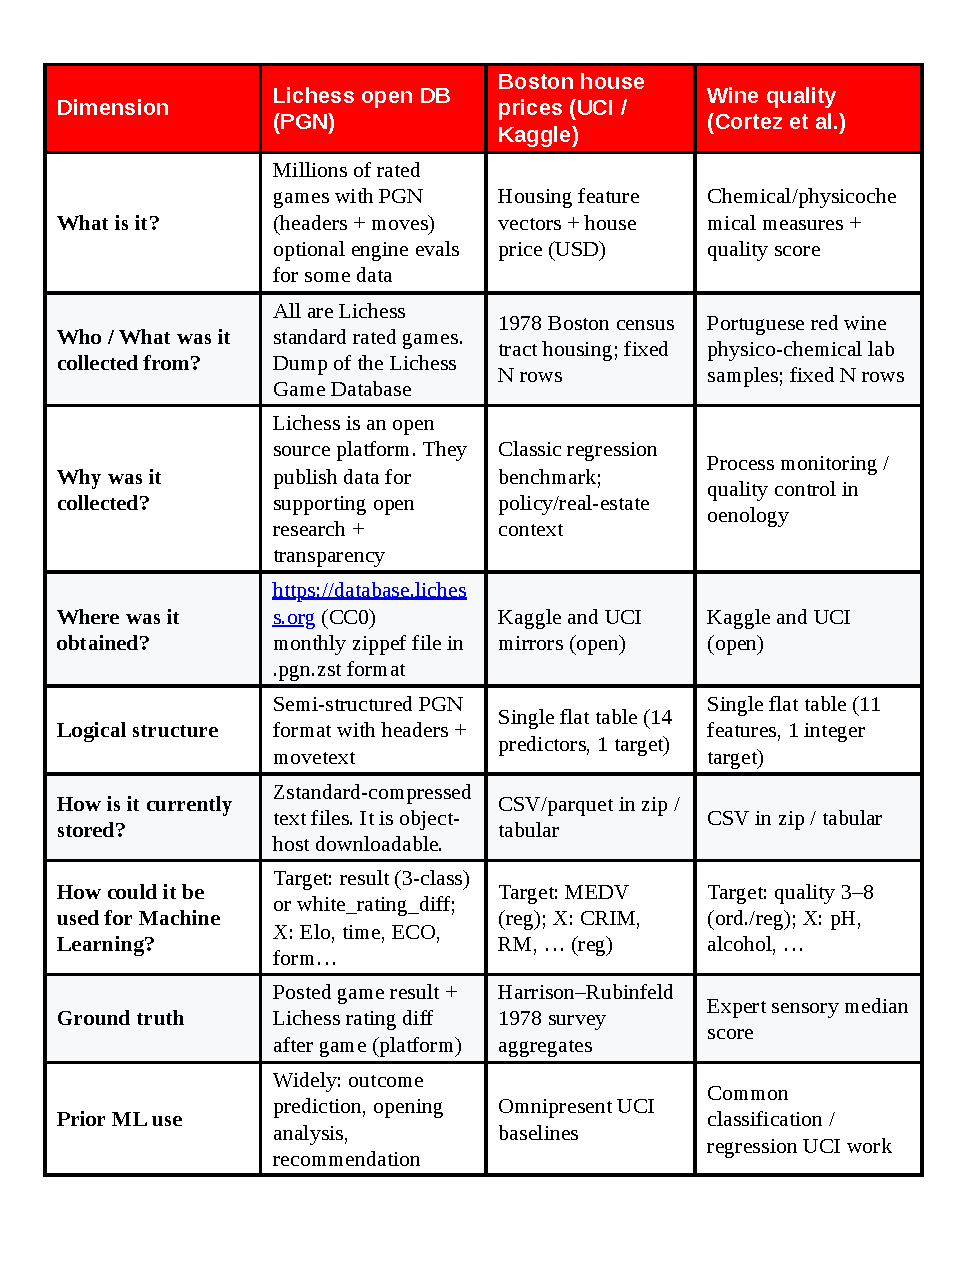
\includegraphics[width=\linewidth,keepaspectratio]{step1.pdf}
  \caption{Candidate dataset comparison across provenance, structure, storage, and supervised-learning affordances.}
  \label{fig:step1-candidate-matrix}
\end{figure}

Competitive platforms and public benchmarks offer contrasting source-data profiles for supervised
learning. This chapter evaluates three candidates transactional game telemetry, tabular chemistry
data, and census-derived housing attributes---and selects one for downstream pipeline design.
\Cref{fig:step1-candidate-matrix} summarises three candidates across provenance, structure, storage, and supervised-learning affordances.

\section[Dataset one]{Candidate dataset \textnumero\,1}
\label{sec:dataset-one}

\textbf{Lichess} ships monthly rated \texttt{.pgn.zst} archives (\url{https://database.lichess.org/}) with outcomes, clocks, ratings, openings, and SAN movelists under a \textsc{cc}0 licence~\cite{lichess_open_database}; see~\cref{app:lichess-open-database} for inventory.
Headers plus ordered moves form the logical model; physically the corpus is compressed text shards, not ready-made tables.
Supervised targets include game outcome (\texttt{[Result]}) and rating-based signals from pre-game headers (\cref{fig:lichess-pgn-sample}).

\begin{table}[h]
\centering
\caption{Lichess Chess Games (2013–present)}
\begin{tabular}{|p{0.25\textwidth}|p{0.65\textwidth}|}
\hline
\textbf{Field} & \textbf{Description} \\
\hline
Source & \url{https://database.lichess.org/} \\
\hline
Format & .pgn.zst (compressed Portable Game Notation using Zstandard) \\
\hline
Size & Jan 2013: 17.8 MB compressed. \\
      & Total: 2.49 TB, 7,863,012,346 games. \\
\hline
Features & Event, Site, Date, Round, White, Black, Result, UTCDate, UTCTime, \\
          & WhiteElo, BlackElo, WhiteRatingDiff, BlackRatingDiff, WhiteTitle, \\
          & ECO, Opening, TimeControl, Termination, \%eval, \%clk, \ldots \\
\hline
Target Variable & Game Outcome (win/loss/draw) \\
\hline
Time Period & January 2013 to present (monthly releases) \\
\hline
\end{tabular}
\end{table}

\section[Dataset two]{Candidate dataset \textnumero\,2}
\label{sec:dataset-two}

\textbf{Wine Quality}~\cite{Cortez2009wine,UCIWineQuality} is a static CSV of physicochemical assays with ordinal quality scores collected from Portuguese wine samples.
Flat relational structure and simple ingestion suit tabular baselines, but the corpus is small, stale, and lacks the temporal refresh needed for operational MLOps practice (\cref{fig:uci-wine-schema}).

\begin{table}[h]
\centering
\caption{Wine Quality (UCI)}
\begin{tabular}{|p{0.25\textwidth}|p{0.65\textwidth}|}
\hline
\textbf{Field} & \textbf{Description} \\
\hline
Source & \url{https://archive.ics.uci.edu/dataset/186/wine+quality} \\
\hline
Format & CSV \\
\hline
Size & 89 KB \\
\hline
Features & fixed\_acidity, volatile\_acidity, citric\_acid, residual\_sugar, \\
          & chlorides, free\_sulfur\_dioxide, total\_sulfur\_dioxide, density, \\
          & pH, sulphates, alcohol \\
\hline
Target Variable & quality (score) \\
\hline
Time Period & 2009 \\
\hline
\end{tabular}
\end{table}



\section[Dataset three]{Candidate dataset \textnumero\,3}
\label{sec:dataset-three}

\textbf{Boston housing}~\cite{HarrisonRubinfeld1978,UCIBostonHousing} comprises census and environmental attributes for Boston-area tracts with median home value (\texttt{MEDV}) as a continuous regression target.
The fixed flat-file schema suits classic tabular baselines rather than transactional chess telemetry and offers limited scale for ingestion, validation, and feature-store design (\cref{fig:boston-housing-sample}).

\begin{table}[h]
\centering
\caption{Boston Housing}
\begin{tabular}{|p{0.25\textwidth}|p{0.65\textwidth}|}
\hline
\textbf{Field} & \textbf{Description} \\
\hline
Source & \url{https://lib.stat.cmu.edu/datasets/boston} \\
\hline
Format & Fixed‑width formatted text file \\
\hline
Size & 506 rows × 14 columns, ~27 KB (compressed ~7 KB) \\
\hline
Features & CRIM, ZN, INDUS, CHAS, NOX, RM, AGE, DIS, RAD, TAX, \\
          & PTRATIO, B, LSTAT \\
\hline
Target Variable & MEDV (median value of owner‑occupied homes in \$1000’s) \\
\hline
Time Period & 1970s \\
\hline
\end{tabular}
\end{table}

\section{Chosen dataset and justification}
\label{sec:chosen-dataset}

We select the Lichess open database for MLOps development due to its sheer volume, scale, embedded labels, \textsc{cc}0 licensing, and monthly refresh.  Lichess dataset clearly outweighes the simpler study purpose datasets like Wine Quality and Boston housing baselines (\cref{sec:dataset-two,sec:dataset-three,fig:step1-candidate-matrix}). Additionally, Lichess Data is produced from a live platform with a large user base, so it has a real-world provenance and operational profile that suits and provides ample direction for learning opportunity in MLOps pipeline design and Data Management. 

% Following are table summarising the operational profile of the Lichess dataset which further supports this selection choice (\cref{tab:lichess-operational-profile,tab:lichess-ml-features}).


% \begin{table}[htbp]
%   \centering
%   \caption{Operational profile of the selected Lichess corpus.}
%   \label{tab:lichess-operational-profile}
%   \small
%   \setlength{\tabcolsep}{4pt}
%   \renewcommand{\arraystretch}{1.15}
%   \begin{tabular}{@{}>{\raggedright\arraybackslash}p{0.21\linewidth}
%                   >{\raggedright\arraybackslash}p{0.73\linewidth}@{}}
%     \toprule
%     Dimension & Assessment\\
%     \midrule
%     Volume and velocity &
%       Approximately \(7.68\times10^{9}\) rated games in \(\sim\)2.43\,TB of Zstandard-compressed PGN (\cref{app:lichess-open-database}).
%       Non-cumulative monthly dumps add on the order of \(5\times10^{7}\)--\(10^{8}\) games per month.\\
%     Schema complexity &
%       No fixed relational schema
%       Movetext is encoded in SAN, requiring parse or tokenisation pipelines.
%       Field inventories evolve gradually---newer months introduce headers such as \texttt{[Accuracy]} or \texttt{[Termination]} absent from early releases.\\
%     Data quality and sparsity &
%       Mix of elite (\(\geq 2500\) Elo) and casual pairings; optional tags may be absent (\texttt{[Opening]} unset for off-book positions).
%       Outcome priors are tempo-dependent: draws account for \(<2\%\) of bullet (\texttt{1+0}) games but approach \(10\)--\(15\%\) under classical controls.
%       Rating-delta targets are noisy when provisional ratings apply to new accounts.\\
%     Temporal and causal structure &
%       UTC timestamps support chronological splits and back-testing; monthly partitions suit incremental ingestion.
%       Player-level correlation violates independence for rating-change targets---splits should respect time or player identifiers, not naive random shuffling.\\
%     Operational limitation &
%       Bulk exports are post hoc monthly artefacts, not a live stream.
%       Near-real-time inference would require a complementary WebSocket feed in addition to the open-database cadence.\\
%     \bottomrule
%   \end{tabular}
% \end{table}

\subsection{Supervised modelling}
\label{sec:supervised-modelling}

The primary supervised task is \emph{pre-game outcome prediction}: given features available before the first move (ratings, time control, variant), estimate whether White wins, Black wins, or the game is drawn, a three-class classification problem with ground truth in \texttt{[Result]} (\texttt{1-0}, \texttt{0-1}, \texttt{1/2-1/2}).
% \Cref{tab:lichess-ml-features} maps labels, baseline predictors, PGN sources, and modelling caveats.

% \begin{table}[htbp]
%   \centering
%   \caption{Machine learning features and labels derivable from the Lichess dataset.}
%   \label{tab:lichess-ml-features}
%   \footnotesize
%   \setlength{\tabcolsep}{3.5pt}
%   \renewcommand{\arraystretch}{1.12}
%   \begin{tabular}{@{}>{\raggedright\arraybackslash}p{0.13\linewidth}
%                   >{\raggedright\arraybackslash}p{0.27\linewidth}
%                   >{\raggedright\arraybackslash}p{0.28\linewidth}
%                   >{\raggedright\arraybackslash}p{0.26\linewidth}@{}}
%     \toprule
%     Role & ML construct & Principal sources & Ground truth / caveats\\
%     \midrule
%     Label &
%       Game outcome (White win\,/\,draw\,/\,Black win). &
%       \texttt{[Result]} (\texttt{1-0}, \texttt{1/2-1/2}, \texttt{0-1}). &
%       Terminal result on record is the supervised ground truth; validate parsing across shards; expect tempo-dependent class skew.\\
%     Feature &
%       Relative strength / pairing imbalance. &
%       \texttt{[WhiteElo]}, \texttt{[BlackElo]}, derived rating gap (and titles if headers include them). &
%       Ratings proxy skill but drift over months; handle missing or placeholder (\texttt{?}) values for unrated or anonymous games.\\
%     Feature &
%       Clock format / tempo regime. &
%       \texttt{[TimeControl]}; chess variant headers when analysing non-standard rulesets. &
%       Strong behavioural prior; bucket bullet\,/\,blitz\,/\,rapid\,/\,classical during preprocessing for stability.\\
%     Feature &
%       Opening / early trajectory signal. &
%       First \(N\) half-moves from the SAN movelist; optional \texttt{[ECO]} when present in headers. &
%       Very high cardinality; employ hashing, embeddings, or clustering; beware transpositions if enriching from external opening tables.\\
%     Feature &
%       Length / pace proxies. &
%       Ply count from SAN tokens; optional \texttt{\%clk} timestamps alongside \texttt{[UTCDate]} / \texttt{[UTCTime]} comments when exported. &
%       Signals complexity or time trouble; clock commentary is shard-dependent---treat as optional enrichment, not assumed globally.\\
%     Feature &
%       Termination channel. &
%       \texttt{[Termination]} when present (mate, resignation, timeout, etc.). &
%       Post-game metadata; exclude from pre-game predictors or treat as diagnostic only---often correlated with outcome.\\
%     Feature &
%       Position-derived telemetry (advanced). &
%       Parsed positions (material balance, mobility); optional engine evaluations via offline joins. &
%       Highest fidelity but requires full SAN parsing or auxiliary computation; heavier engineering than header-only baselines.\\
%     \bottomrule
%   \end{tabular}
% \end{table}

\chapter{Data Storage Plan}
\label{ch:storage-planning}
This chapter focuses on the data decisions taken while designing the MLOps pipeline. Further this section also discusses about the physical and logical structure of the dataset showcasing how the current design decisions helps in making the optimal for data analytics and downstream meaching learning tasks too.  

% Chapters~\cref{ch:candidate-datasets}--\cref{ch:pipeline-planning} fix corpus plus DAG scope; landing and joins only~\cite{lichess_open_database}.

\section{Data Source}
\label{sec:storage-source}
The data is from Lichess platform which is an open source alternative version of chess.com for playing chess online. Lichess publishes its entire games from database for public use at \url{database.lichess.org}. It is a bulk file which can be downloaded over HTTPS. Each month a single compressed file is published alongside a SHA256 checksum for validation. This project downloads those files, verifies it, and lands it in the object store named MinIO. 

\subsection{Physical Storage}
\label{sec:storage-provenance}
The raw file downloaded from Lichess which is downloaded and stored in object storage is a compressed PGN file using Zstandard. Zstandard (zstd) was chosen by Lichess because of its balance for compression ration and decompression speed. Once decompressed, the plain-text PGN is roughly five times larger. A typical month goes from ~20 GB to ~100 GB. The raw file remains in the lake as a single immutable object with no transformation is done at this stage.

% \texttt{database.lichess.org} publishes monthly \texttt{.pgn.zst} shards plus checksum pairs; verified copies sit in MinIO with inventory in~\cref{app:lichess-open-database}~\cite{lichess_open_database}.

\subsection{Logical Storage}
\label{sec:logical-storage}
The PGN format is semi-structured file format for storage chess games with metadata. There is no enforeced schema but the structure repeats reliably. Every game is a block of following components:

\begin{enumerate}
    \item A set of headers
    \item An empty line in between
    \item The move list in Standard Algebraic Notation. Some games also contains evaluation from stockfish chess engine.
\end{enumerate}



Logically we can think of the dataset as two nested entities.
\begin{enumerate}
 \item \textbf{Game:} Fixed attributes (date, players, result, opening, etc.).
 \item \textbf{Move:} An ordered list of half-moves, each carrying a move number, SAN notation, UCI coordinates, evaluation, and clock remaining. 
\end{enumerate}

The cardinality is one game to zero-or-many moves.

\section{Ingested Data Storage}
\label{ingested_data_storage}
After extraction and loading, the raw \texttt{.zst} object is transformed into a set of Parquet tables arranged in a star schema. I follow an ELT pattern: the compressed file lands unchanged in MinIO first (load), then Apache Spark reads from object storage to parse and shape the data (transform), and the curated tables are written to MinIO as Parquet and loaded into DuckDB for analytics.


\subsection{Why Parquet?}
\begin{itemize}
    \item Fast aggregations (scans only the columns needed).
    \item High compression (columns hold similar data).
    \item Predicate push-down with Spark/DuckDB (partition pruning on year/month).
\end{itemize}

\subsection{Why MinIO?}
It keeps compute and storage separate, allows direct S3-compatible reads from Spark, DuckDB, and Feast, and the raw bucket gives a permanent, immutable copy for reprocessing.

\subsection{Logical structure (Star Schema)}
The processed data is modelled as a star schema centred on \texttt{fact\_games}. The design is shown in \cref{fig:dataset-one-logical-erd} as a crow-foot ERD.

\begin{figure}[htbp]
  \centering
  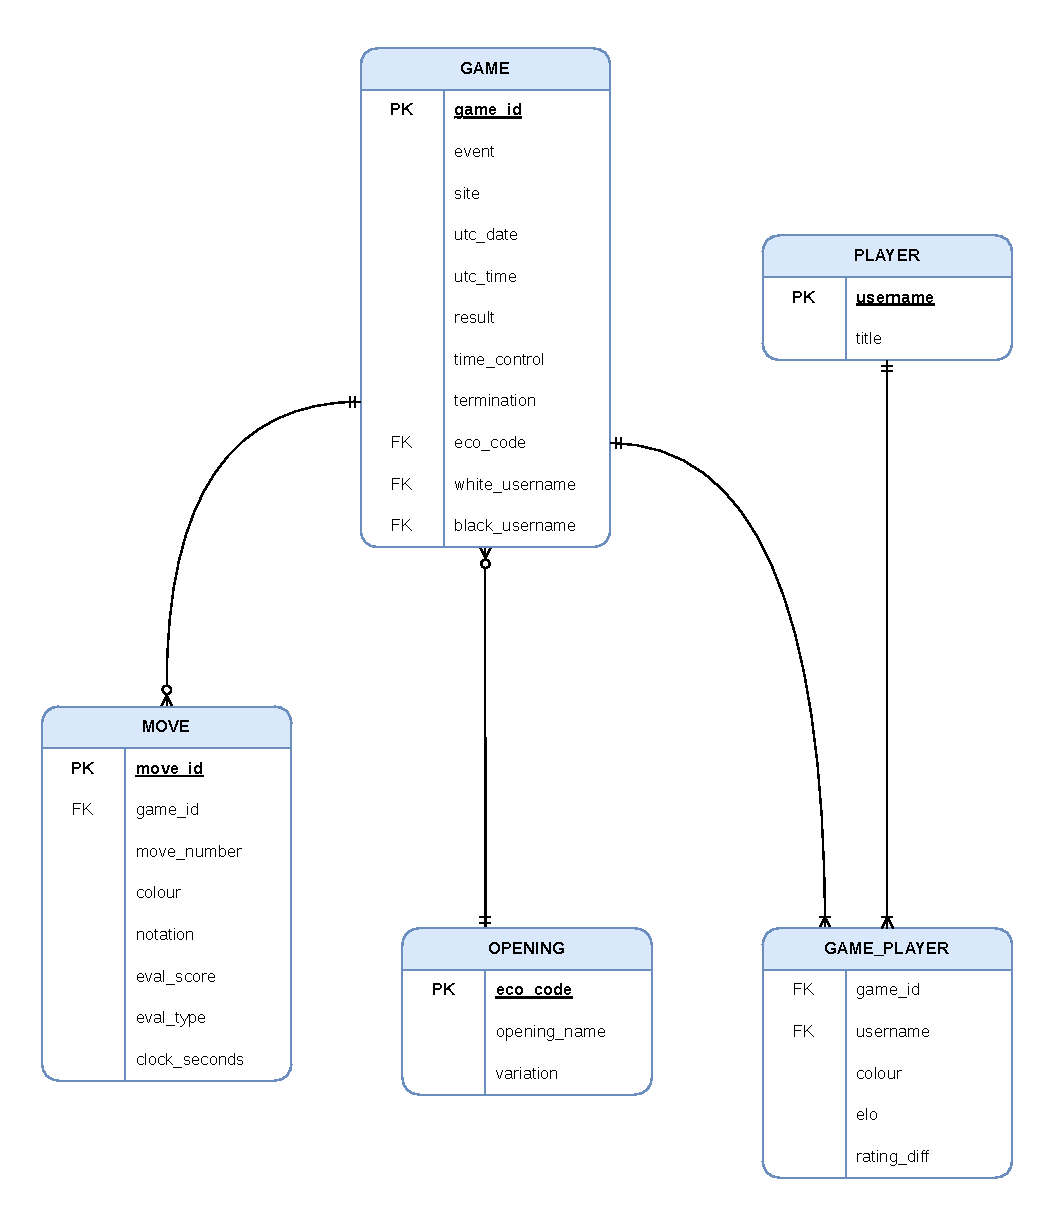
\includegraphics[width=0.95\linewidth,height=0.85\textheight,keepaspectratio]{erd}
  \caption{Star schema for processed Lichess data: a central fact table of games with dimensions for players, openings, and dates.}
  \label{fig:dataset-one-logical-erd}
\end{figure}



\subsection{Justification for the star schema}
The star schema was chosen because it directly supports the two main consumer groups in the pipeline:


\begin{table}[htbp]
    \centering
    \renewcommand{\arraystretch}{1.5}
    \begin{tabular}{|p{0.3\textwidth}|p{0.65\textwidth}|}
        \hline
        \textbf{Need} & \textbf{How the star schema meets it} \\ \hline
        ML feature engineering (Feast) & Feast works with entity keys; the fact table and dimensions can be mapped to Feast FeatureViews with simple joins on player, opening, or date keys. Point-in-time joins are straightforward. \\ \hline
        Analyst / Data Scientist notebooks & A single join from the fact table to a dimension is enough for most queries; no complex multi-table logic. \\ \hline
        Storage efficiency & Player attributes (username, title) are stored once, not repeated per game. Parquet columnar compression reduces the footprint further. \\ \hline
        Incremental monthly loads & Partitioning on year/month means new months are appended; dimensions are updated with a merge without rewriting the whole fact table. \\ \hline
        Data quality checks & Each table can have a dedicated Great Expectations suite (e.g., null checks on fact columns, uniqueness on dimension keys). \\ \hline
    \end{tabular}
\end{table}

\section{Benefits, drawbacks and Mitigation of the star schema}
The star schema model is straightforward to communicate to both engineers and data scientists because breaking the dataset into games, players, openings, and dates maps naturally to the chess domain. By using this approach, we avoid the massive data duplication that typically plagues a single, wide table. This structure also perfectly complements the write-once, read-many nature of historical chess data. While queries requiring multiple dimensions do need joins, the dimensions are relatively small, and engines like DuckDB or Spark manage these columnar joins quite efficiently. We accepted a minor bit of redundancy, such as storing the \texttt{last\_known\_elo} directly in the \texttt{dim\_player} table instead of constantly recalculating it from the fact table, simply because it makes looking up current ratings significantly faster. Finally, although evolving the schema—like adding a brand new dimension—demands careful coordination, using Parquet makes this manageable by supporting schema merging and allowing new dimensions to be introduced independently over time.

\section{Alternative structure}
\begin{table}[htp!]
    \centering
    \begin{tabular}{|p{3cm}|p{3.5cm}|p{4.5cm}|p{3.5cm}|}
        \hline
        \textbf{Approach} & \textbf{Upside} & \textbf{Downside \& Mitigation} & \textbf{Why not chosen} \\ \hline
        One Big Table & Zero joins, simple CSV & Huge duplication, brittle schema, breaks temporal correctness & Duplication and temporal fidelity risk too high \\ \hline
        Star Schema (chosen) & Familiar, fits Feast, good compression, incremental & Joins needed; mitigated by columnar scans and small dimensions & --- \\ \hline
        Snowflake & Even less redundancy in dimensions & Extra joins for minimal gain (shallow ECO hierarchy) & Complexity doesn’t pay off \\ \hline
        3NF relational & Clean updates, no anomalies & Many‑table joins hurt read speed at scale & Append‑heavy workload; read performance more important \\ \hline
        Medallion layers & Clear quality gates & Overlaps with raw/processed bucket split & Redundant; our raw bucket already provides the “bronze” layer \\ \hline
    \end{tabular}
\end{table}


\section{Extraction, Loading, and Transformation (ELT)}
I follow an ELT pattern because the heavy transformation happens after the data lands in the object store MinIO.

\begin{figure}[htbp]
  \centering
  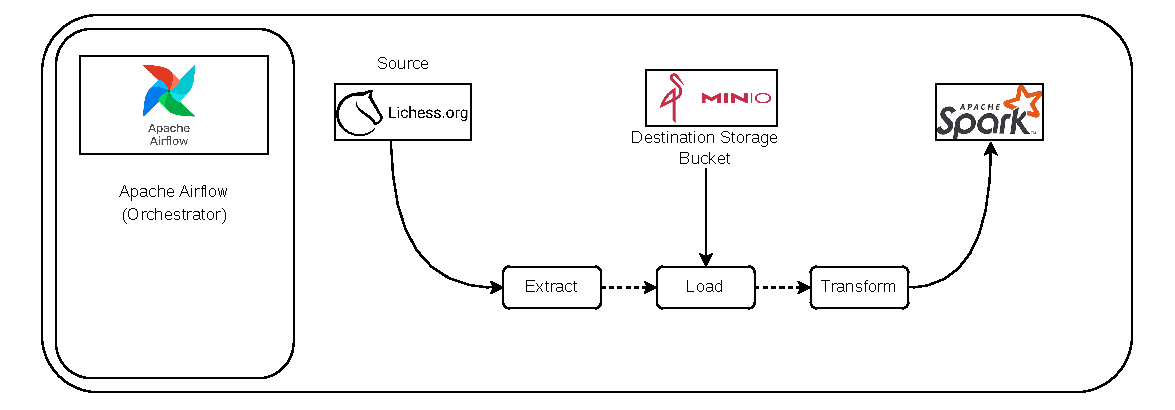
\includegraphics[width=\linewidth,height=0.55\textheight,keepaspectratio]{elt.pdf}
  \caption{ELT pattern with object storage.}
  \label{fig:elt-flow}
\end{figure}



\subsection{Extract}
An Airflow DAG fetches each monthly \texttt{.pgn.zst} file from Lichess over HTTPS and checks it against the published SHA256 checksum. A mismatch fails the task and triggers an alert.

\subsection{Load}
The verified file lands in MinIO at \texttt{s3://lichess-raw/pgn/...} without decompression or parsing. It stays there as an immutable archive until Spark reads it.

\subsection{Transform}
PySpark streams the \texttt{.zst} object from MinIO, decompresses it in-flight, and parses games with a python-chess UDF. Headers and derived fields (e.g.\ move count) go to \texttt{fact\_games}; half-moves, engine evaluations, and clock times optionally go to \texttt{fact\_moves}. Distinct players, openings, and dates are merged into \texttt{dim\_player}, \texttt{dim\_opening}, and \texttt{dim\_date}. Curated tables are written to \texttt{s3://lichess-processed/} as Parquet, with fact tables partitioned by year and month.

\subsection{Validation}
Great Expectations runs a checkpoint on each new partition (schema, null rates, value bounds). Partitions that pass are released to Feast and analyst notebooks.


\chapter{Final MLOps and Data Engineering Pipeline Plan}
\label{ch:final-pipeline-planning}


This section presents the planned data analytics pipeline for ingesting, processing, and
serving the Lichess dataset to two classes of consumer: (1) Analysts performing ad hoc
queries and generating reports via SQL/notebooks and (2) An
automated machine learning pipeline for supervised model training and serving.


\begin{figure}[htbp]
  \centering
  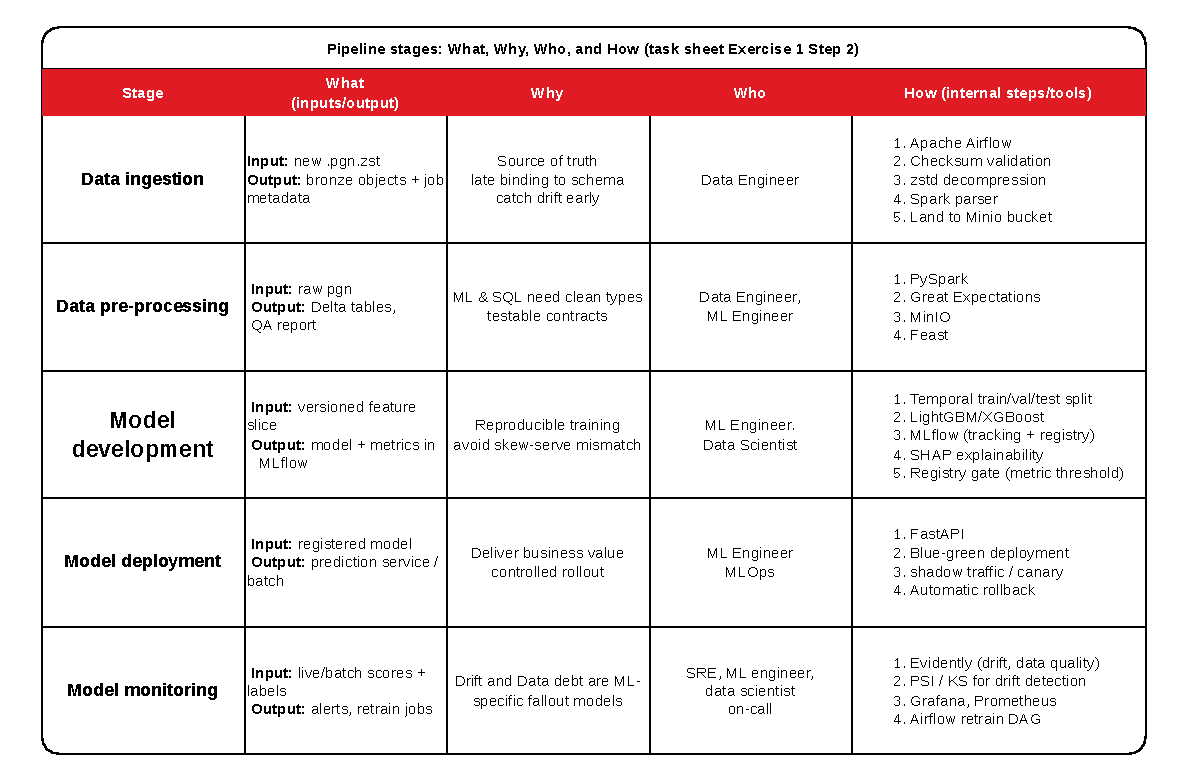
\includegraphics[width=\linewidth,keepaspectratio]{whowhatandhow.pdf}
  \caption{Pipeline stages: What, Why, Who, and How for each stage of the MLOps workflow.}
  \label{fig:pipeline-whowhatandhow}
\end{figure}


\begin{figure}[htbp]
  \centering
  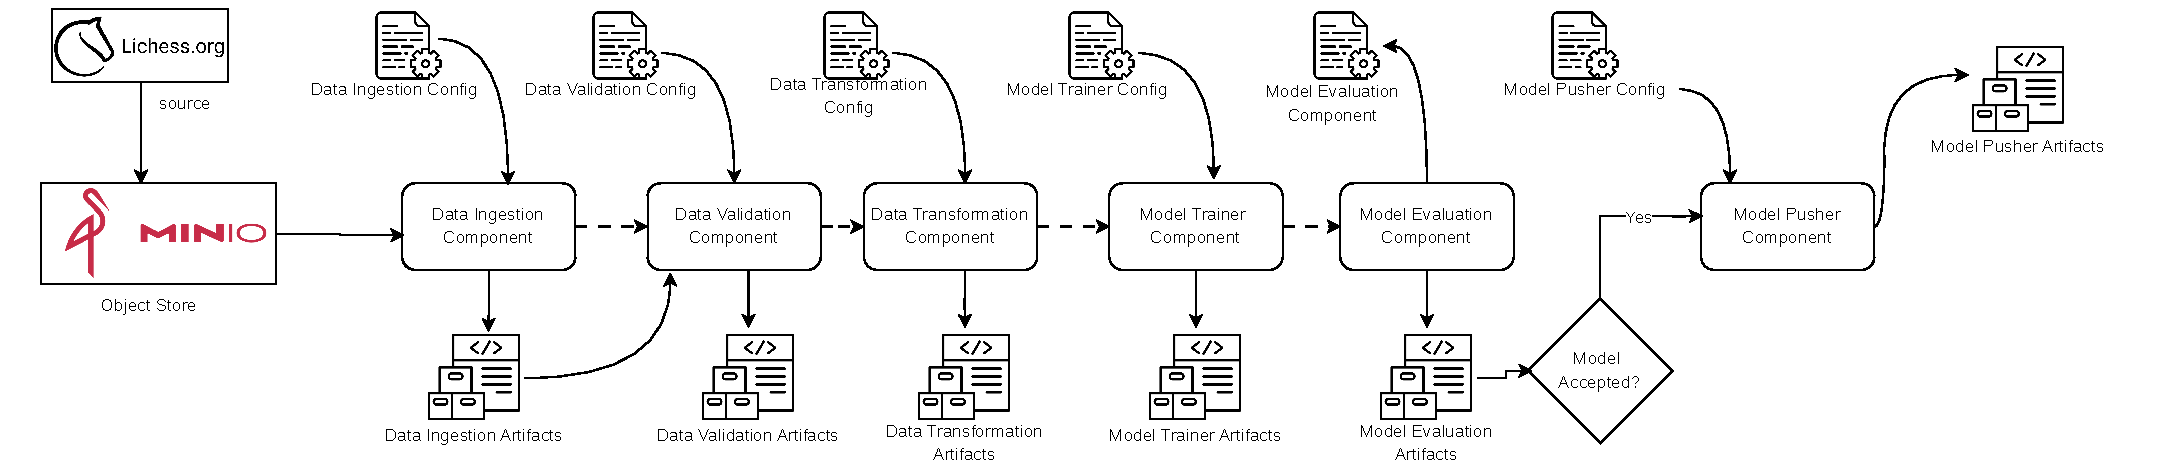
\includegraphics[width=\linewidth,height=0.92\textheight,keepaspectratio]{arch_diag.pdf}
  \caption{End-to-end MLOps pipeline divided in terms of configuration, artefacts, and components.}
  \label{fig:mlops-pipeline}
\end{figure}

\section{Data ingestion}
\label{sec:stage-ingestion}

\begin{figure}[htbp]
  \centering
  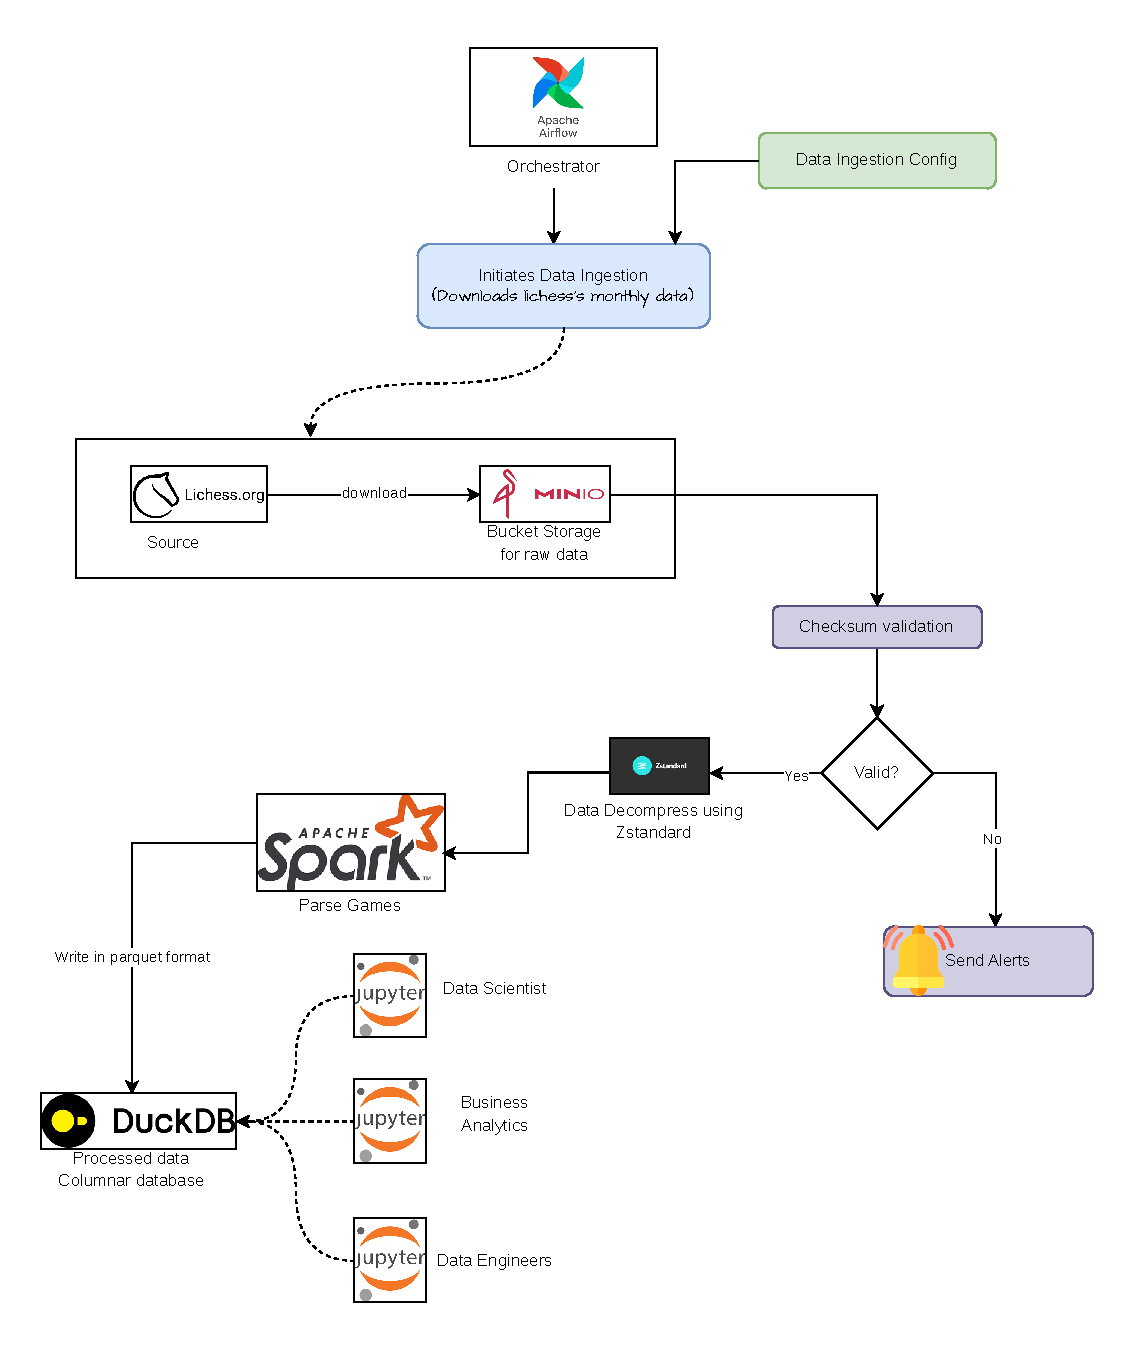
\includegraphics[width=\linewidth,height=0.85\textheight,keepaspectratio]{dataIngestion.pdf}
  \caption{Data ingestion (\emph{extract} and \emph{load}): the orchestrator applies ingestion config, downloads the monthly \texttt{.pgn.zst} from Lichess to a raw-data bucket in MinIO, and validates checksums before landing the blob unchanged; checksum failures trigger alerts.}
  \label{fig:data-ingestion}
\end{figure}

This pipeline automates the ingestion of Lichess's monthly public game data using the Apache Airflow orchestrator. This stage covers the \emph{extract} and \emph{load} steps of the ELT pattern (\cref{fig:elt-flow}; \cref{ch:storage-planning}): the monthly shard is downloaded over HTTPS, its integrity is verified (SHA256), and the compressed file is landed in MinIO as a single immutable object with no parsing or reshaping.

Decompression, PGN parsing, and curated star-schema Parquet are performed in preprocessing (\cref{sec:stage-preprocessing}). We use MinIO as an S3-compatible store for raw and processed data; Parquet partitions in the processed bucket feed MariaDB and downstream analysts and ML tooling.

\section{Data pre-processing}
\label{sec:stage-preprocessing}

In preprocessing, a PySpark job implements the \emph{transform} step: it reads the raw \texttt{.zst} stream from MinIO, decompresses the Zstandard payload, parses each game into header-derived fields (and optionally move rows), builds the star-schema DataFrames (\texttt{fact\_games}, dimensions, optionally \texttt{fact\_moves}), and writes partitioned Parquet to the processed bucket.

After Spark writes those star‑schema Parquet files to MinIO, they are loaded into MariaDB, the columnar database which offers fast read. The tables containing the dimensions and the fact games are stored in MariaDB, so that fast SQL can be used for both validation. Great Expectations checkpoint is performed on the whole MariaDB table (or the corresponding Parquet) prior to any split. Verifies columns, data types, null ratios, and ranges of data. The pipeline stops if the validation fails and an alert is sent otherwise, an artefact is created which certifies the data quality. Feast (with MariaDB as its offline store) supports the point in time feature retrieval for the entire historical data. The time-dependent features (e.g., win rate of the players in the last 30 days) are calculated based on only data prior to the game's timestamp to prevent temporal leakage. This will create a feature DataFrame, which now includes all features and the target, split chronologically (e.g., 80 \% train, 20 \% test). Since features were created on the entire data set before the split, both partitions have all columns and there is no problem with “columns missing in training/test”.

\begin{figure}[htbp]
  \centering
  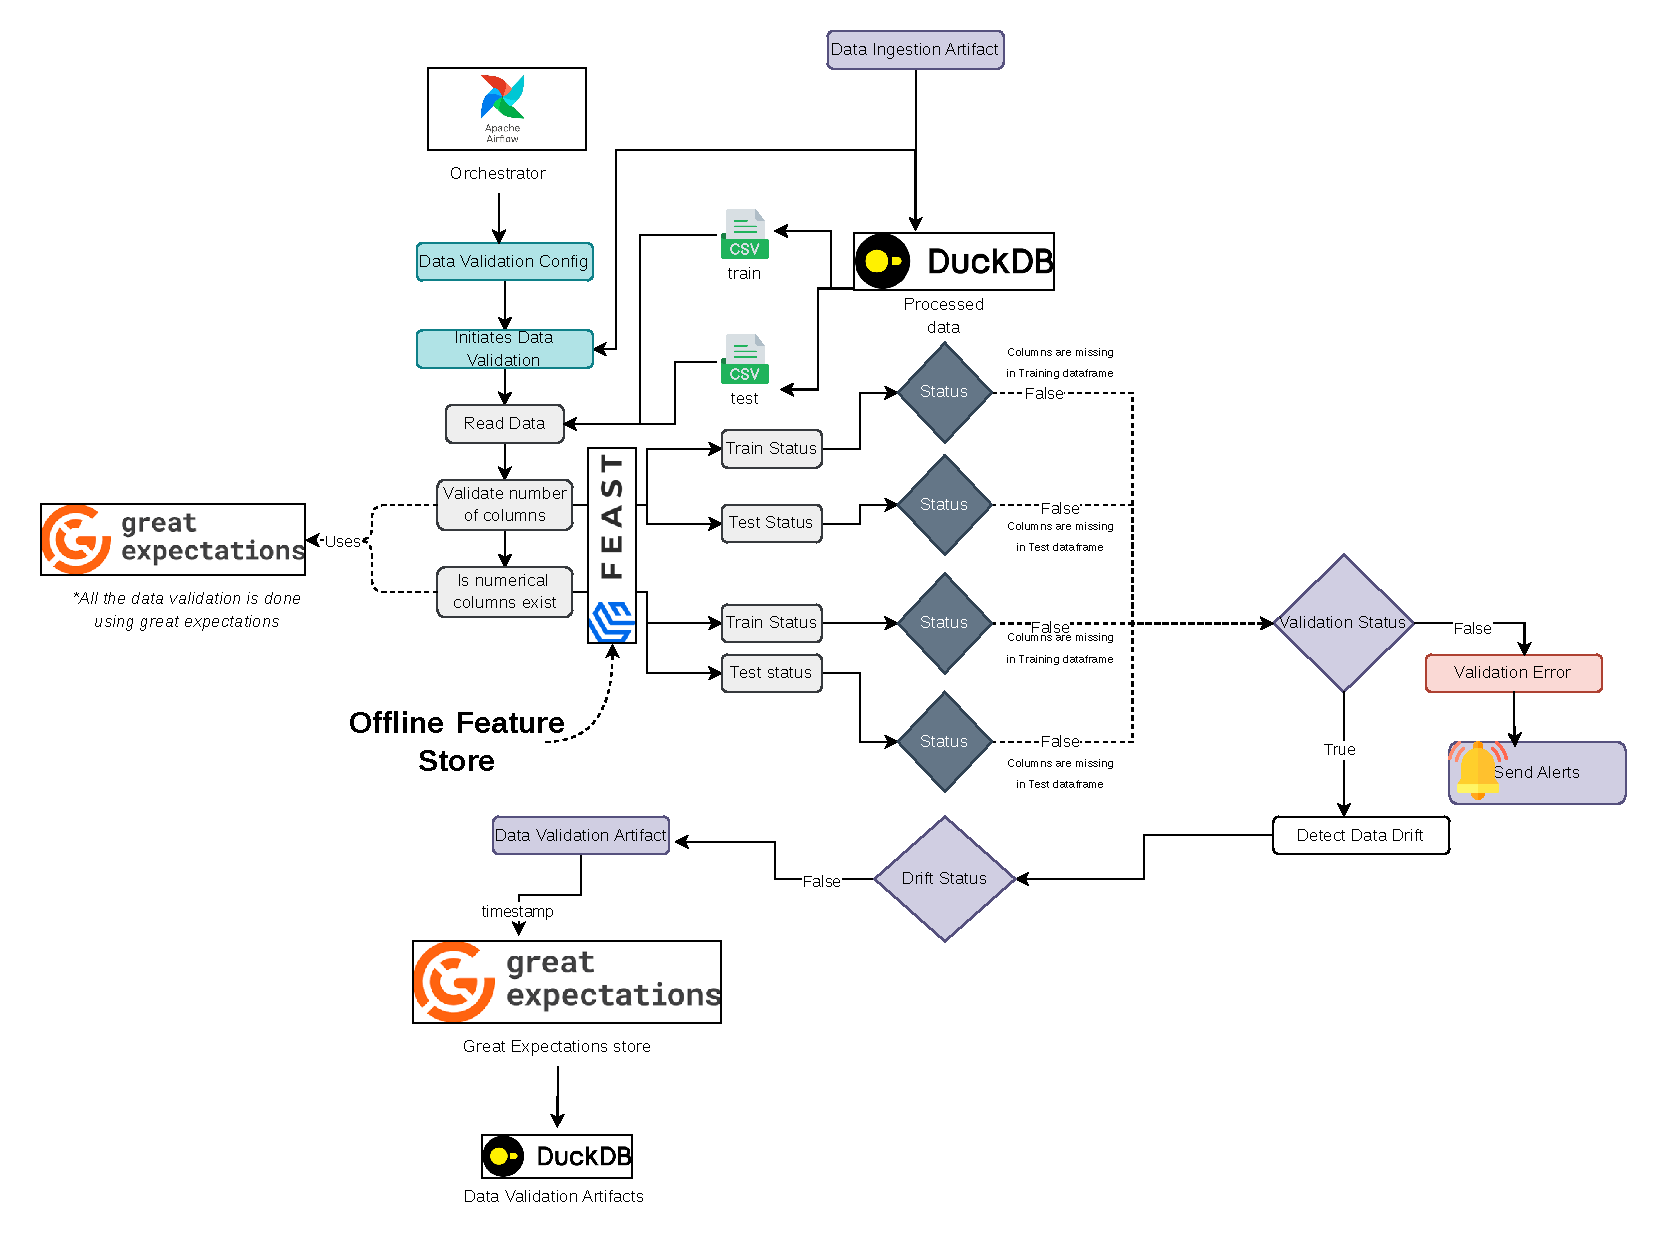
\includegraphics[width=\linewidth,height=0.92\textheight,keepaspectratio]{dataValidation.pdf}
  \caption{Data preprocessing under orchestration: train/test splits are checked for schema completeness and drift; Great Expectations stores validation reports; failures route to alerts and updated artefact keys, while validated processed data feeds an offline feature store.}
  \label{fig:data-validation}
\end{figure}


\section{Model development}
\label{sec:stage-model-dev}

\begin{figure}[htbp]
  \centering
  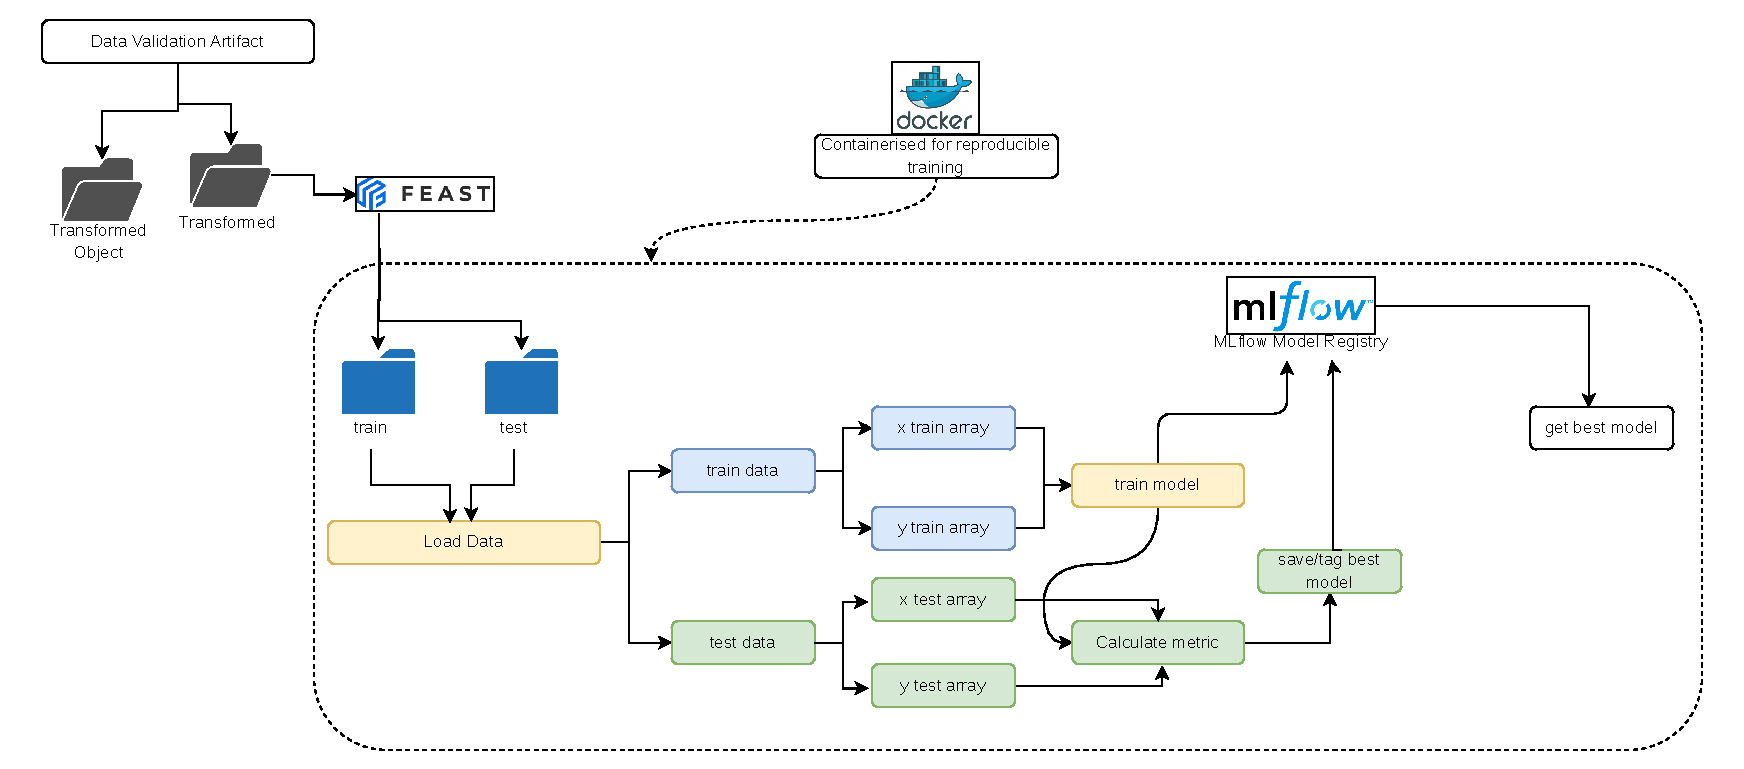
\includegraphics[width=\linewidth,height=0.85\textheight,keepaspectratio]{modelTrainer.pdf}
  \caption{Model training: load train/test arrays from validated artefacts, fit the model, compute metrics, register the best run in MLflow, and retain a containerised, reproducible training environment.}
  \label{fig:plan-model-trainer}
\end{figure}
The model training stage reads  data from database. Here, It uses the Feast for defining the feature from star schema. 

\section{Model deployment}
\label{sec:stage-deployment}

\begin{figure}[htbp]
  \centering
  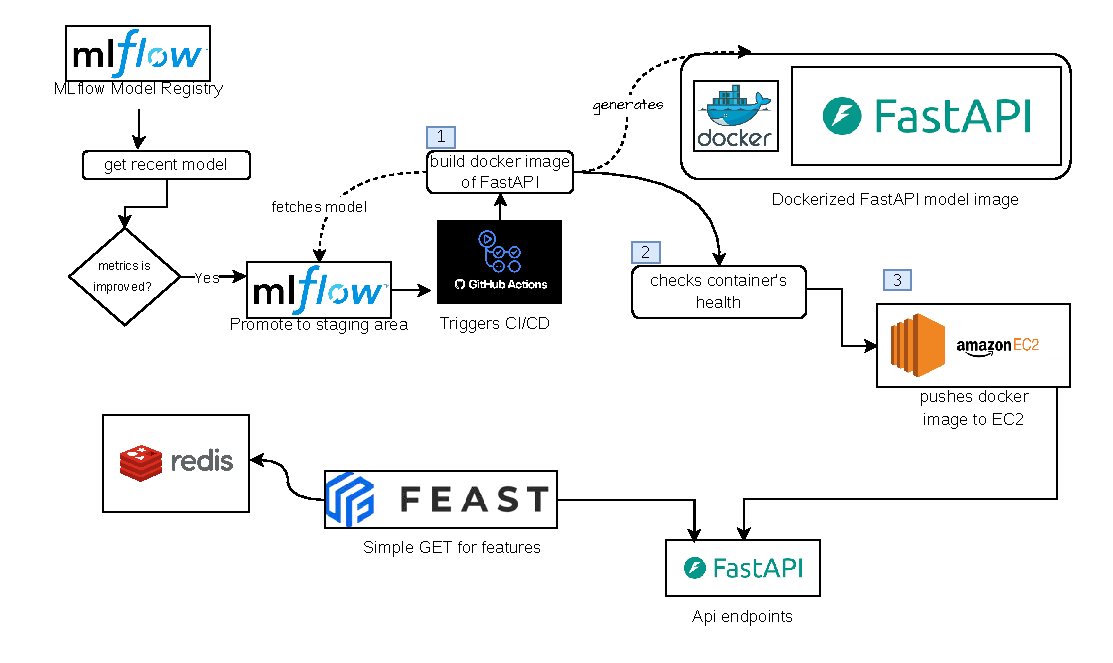
\includegraphics[width=\linewidth,height=0.85\textheight,keepaspectratio]{deployment.pdf}
  \caption{Deployment: promote a recent model from MLflow, build a Dockerised FastAPI image, run health checks, and push to the serving host (e.g.\ EC2); improved metrics can trigger CI/CD to refresh the endpoint.}
  \label{fig:plan-deployment}
\end{figure}

Containers promote only after gates; MLOps owns CI/CD with SecOps image review (\cref{fig:plan-deployment}).
Canary and rollback retag registries; contracts keep serving aligned with preprocessing.

\section{Model monitoring}
\label{sec:stage-monitoring}

\begin{figure}[htbp]
  \centering
  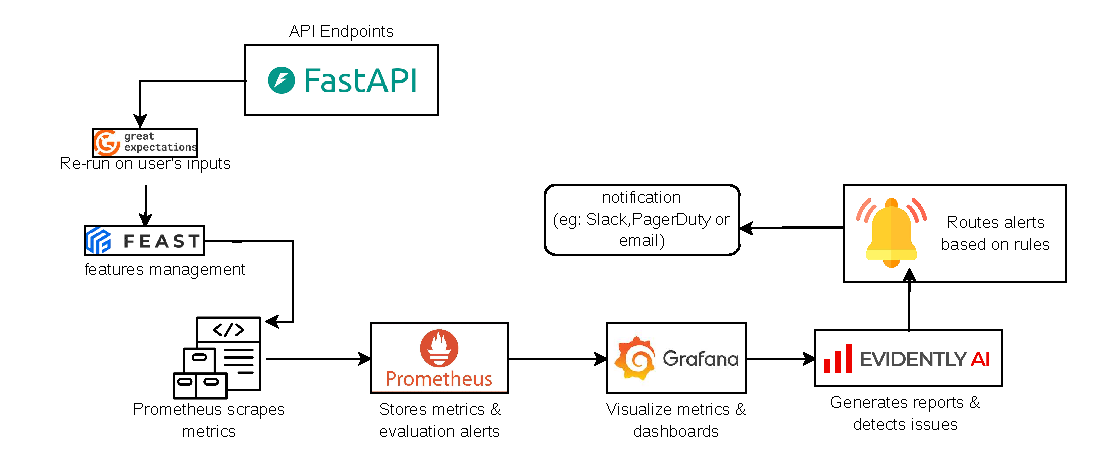
\includegraphics[width=\linewidth,height=0.85\textheight,keepaspectratio]{monitoringObserv.pdf}
  \caption{Monitoring and observability: API metrics scraped by Prometheus, dashboards and automated reports, rule-based routing to Slack/PagerDuty/email, and controlled reruns from user or scheduled inputs.}
  \label{fig:plan-monitoring}
\end{figure}

Production tracks feature drift, latency SLOs, and score error as new months arrive (\cref{fig:plan-monitoring}).
MLOps triages alerts; retrains stay lineage-linked to ingestion batches.


\chapter{Final MLOps and Data Engineering Pipeline Plan}
\label{ch:final-pipeline-planning}

The following sections document the refined pipeline plan as implemented in the LichessOps repository \githubparencite{lichessops_repo}. Each stage follows the What, Why, and How structure from the module brief, aligned with the Task~1 diagrams but updated where implementation constraints changed the approach.

% \subsection{Shared utilities}
% \label{sec:shared}

% Before walking through ingestion or training, it is worth describing the small shared library I extracted once several packages started duplicating the same path logic. Early prototype version had several hard-coded directories after repetitive copy-paste, I centralised the behaviour under \texttt{libs/shared} making the code reusable across different components.

% Each component has configuration loading as shown in figure~\ref{fig:example_libs}. The main use of configuration loading is to  (\codecite{code_config_loader}) walk up from the package until it finds \texttt{pyproject.toml}, then deep-merge \texttt{config/default.yaml} which a config file with a package-specific file. As a developer, This pattern eased up profoundly in configuration management and let me modify MinIO endpoints or MariaDB paths in one place during Docker bring-up without touching Python imports. None of these modules are glamorous, but they made the pipeline development more efficient and less error-prone.


% Object storage helpers in \codecite{code_s3} uses boto3 against MinIO bucket names, upload helpers, and existence checks. \codecite{code_storage_config} turns a month string like \texttt{2024-05} into the right S3 URI or local MariaDB file path so the CLI and Airflow tasks agree on inputs. Logging (\codecite{code_logger}) appends to \texttt{logs/lichess.log} with rotation; when a DAG task failed at 03:00 I could trace it without digging through container stdout alone. I also added a thin \texttt{LichessException} wrapper (see \repo{libs/shared/exception.py}) so CLI failures print file context with helpful information. Exceptions are not user-facing API errors yet, they are just made for developer friendly at this point.



\section{Data ingestion}
\label{sec:ingestion}

\subsection{What}

Data ingestion, in this project mainly involves pulling the monthly Lichess database dump from the public facing website \url{https://database.lichess.org} and storing it in durable object storage so every later stage uses the same bytes. The input is the template URL Lichess publishes from \texttt{database.lichess.org} where we download a Zstandard-compressed PGN file \parencite{zstandard} named \texttt{lichess-YYYY-MM.pgn.zst}. It is a compressed .pgn file which is a standard format to represent the chess game. Each game inside this .pgn file is text with headers (player names, ratings, opening, result). The output of ingestion is not yet a dataframe. it is that validated archive sitting in the \texttt{lichess-raw} bucket \parencite{minio} in a format which is ready for Spark for transformation. 

The visible components are a Python downloader CLI, checksum validation, boto3 uploads, MinIO provisioned via Docker Compose \githubparencite{code_minio_compose}, and Apache Airflow \parencite{apache_airflow} as the scheduler here.

\subsection{Why}

I chose MinIO because PGN and \texttt{.zst} blobs do not map cleanly onto a columnar warehouse table. Object storage treats them as opaque files with cheap immutability and no semantics. I can reprocess April 2024 months later without re-downloading if the raw key still exists. Here, Checksum validation matters due to size of raw file. If the checksum fails then early detection prevents issues. Catching these issues early helps to save time and resources early in the pipeline. 

Airflow runs the DAG on \texttt{0 3 1 * *} (03:00 on the first day of each month) so developer does not need to manually click download when Lichess typically publishes. ELT fits my development setup. Here transformation stays on Spark and DuckDB.

\subsection{How}

The \texttt{lichess\_monthly\_ingestion} DAG \githubparencite{code_airflow_dag} shells out to \texttt{lichess-data}. That Keeps tasks testable from the terminal with the same flags Airflow passes.

On the default path (\texttt{use\_elt=True}):

\begin{enumerate}[nosep]
  \item \textbf{download\_shard}: \texttt{lichess-data download} calls \texttt{download\_month} in \codecite{code_downloader}. The client resumes partial files and can verify SHA256 against Lichess's published sums while bytes still stream.
  \item \textbf{upload\_raw}: \texttt{upload\_raw\_shard} in \codecite{code_upload} pushes to \texttt{s3://lichess-raw/} using \codecite{code_s3}. When \texttt{LICHESS\_STORAGE\_BACKEND=local}, upload is a no-op for laptop-only runs.
  \item \textbf{validate\_shard}: \texttt{validate\_checksum} in \codecite{code_checksum} re-checks integrity. I treat a failure as a hard stop because the DAG should not proceed to Spark on a bad object.
  \item Downstream tasks:  (\texttt{spark\_transform}, \texttt{duckdb\_sync}) consume the raw key which they are preprocessing but depend on this stage finishing cleanly.
\end{enumerate}

Bringing up storage uses the Compose \texttt{core} profile from the repo root \texttt{docker compose --profile core up -d} which also starts MinIO and a one-shot job that creates \texttt{lichess-raw}, \texttt{lichess-processed}, and \texttt{mlflow-artifacts}. Retrieval for later stages is literally an S3 GET on the month prefix which analysts or Spark both read the same URI via \codecite{code_storage_config}.

\begin{figure}[htbp]
  \centering
  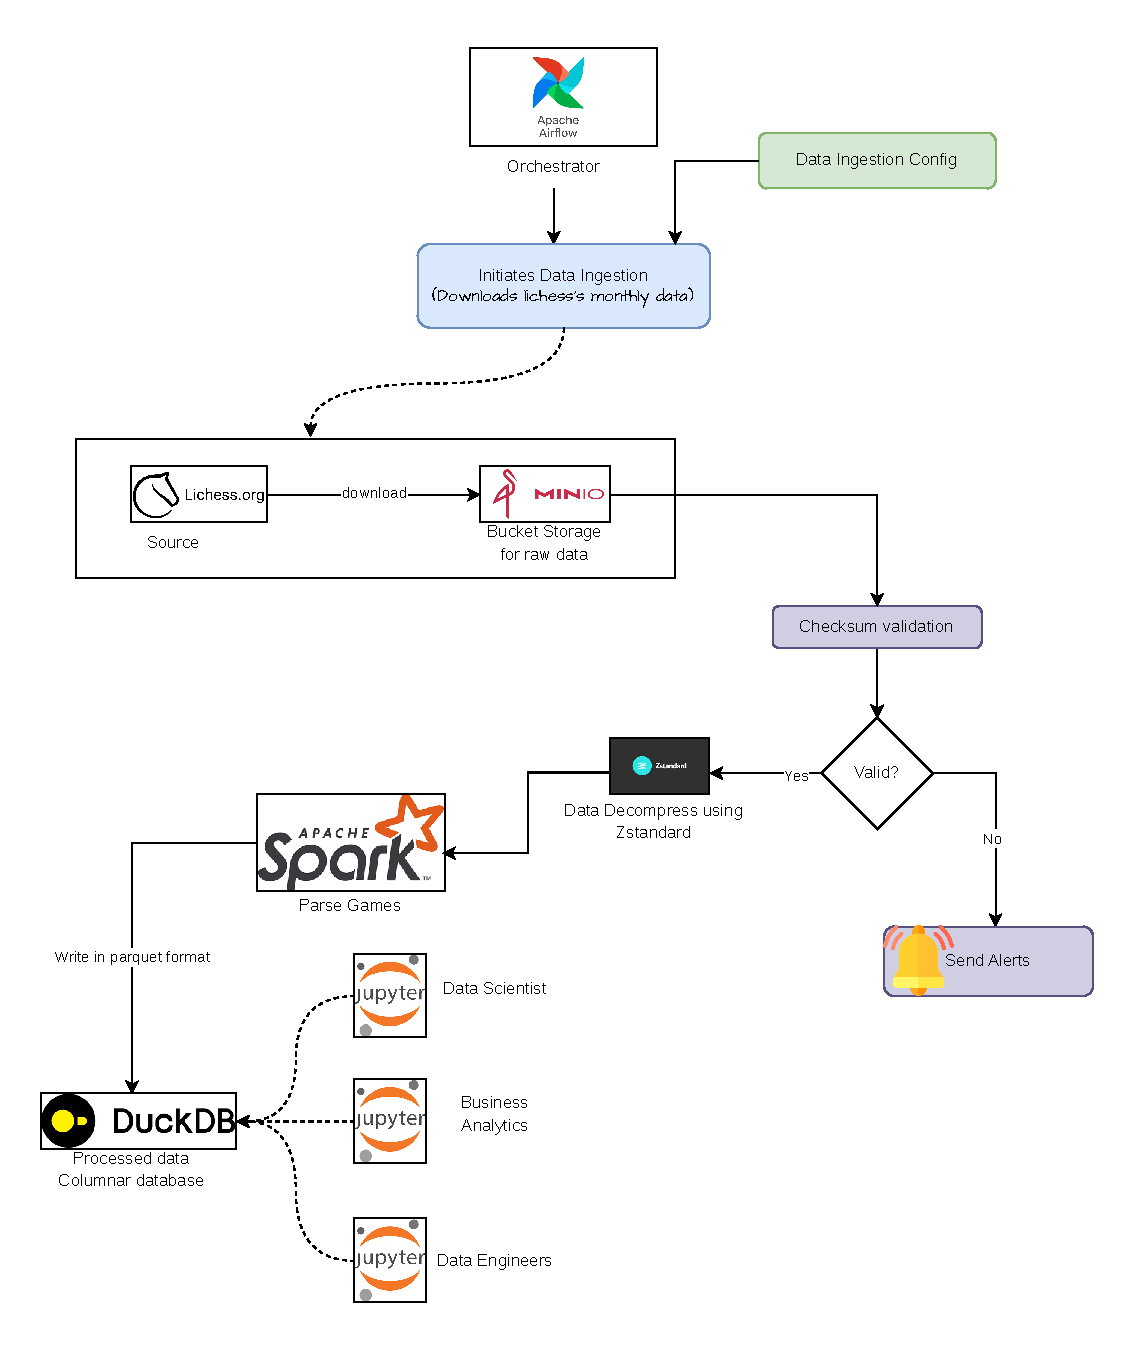
\includegraphics[width=\linewidth,keepaspectratio]{dataIngestion.pdf}
  \caption{Data ingestion: download, checksum validation, and load to MinIO raw bucket.}
  \label{fig:ingestion}
\end{figure}

For retrieval, \texttt{raw\_s3\_uri(month)} returns the full \texttt{s3://} key, which DuckDB's \texttt{httpfs} extension or Spark's S3 configuration consumes. That indirection is how ingestion meets the brief's ``storage and retrieval'' wording even before any ML features exist.

% \textbf{Environment and operations.} Local runs expect \texttt{AWS\_ENDPOINT\_URL=http://localhost:9000} and MinIO credentials matching the Compose file (\texttt{minioadmin} by default). I document the sequence in \texttt{docs/airflow-ingestion.md} and \texttt{docs/lichess-database-downloader.md}; the coursework log captures the intent. First-time Airflow bring-up with the \texttt{orchestration} profile takes several minutes for Postgres and Redis migrations---I learned to start it before the due date, not the night before. Flower (\texttt{flower} profile) helps inspect Celery workers when a task stays queued.

When Lichess rotates CDN behaviour, the downloader reads the monthly index rather than hard-coding URLs. That small robustness mattered because archive paths changed between academic years. 

\section{Data pre-processing}
\label{sec:preprocessing}
Pre-processing turns the chess games into tabular features which later ML libraries can ingest. Inputs are the raw compressed .pgn file using the zstandard compression which are stored in MinIO object storage. After transformation, we store the data into MariaDB columnar storage, after which further validation using great expectations is done. After successful validation, the data made ready for model training using the Feast which is efficient feature store and directly communicates with the columnar database for feature while training. 

\subsection{Tools Used}
PGN is the lingua franca of chess software but a poor format for data analytics efficiency. It consists of variable header keys, multi-line movetext and comments which doesn't fit the tabular format required for efficient data analysis. We store the final artifact file as Apache Parquet \parencite{apache_parquet} which provides us columnar compression and a schema which is compatible across Spark, DuckDB, and Pandas. Here, DuckDB lets run SQL checks such as (\emph{e.g.} ``how many games lack an ECO code?''). For feature storage, I employed Feast.Feast \parencite{feast} handles point-in-time joins so I do not leak future results into past rows, a mistake I almost made when I was first time computing rolling win rates. Great Expectations \parencite{great_expectations} encodes data validation expectations as a checkpoints. When a new monthly data arrives with a schema drift, then the pipeline halts the process instead of training on that drifted data.

\subsection{Implementation}
Following section explains the implementation detail for pre-processing stage with url to github repository as citation for either component or code snippet. Task \texttt{spark\_transform} submits work in \codecite{code_spark_transform}. This job streams the Zstandard payload which parses the headers into structured fields and builds the \texttt{fact\_games} and dimension tables. \texttt{preprocess\_features} executes in ten stages defined in \codecite{code_transforms}. \codecite{code_feast_split} materialises those cleaned games into features with timestamps, then it applies an train test splitting of dataset. \texttt{validate\_ge} invokes \codecite{code_ge_runner}. Failed expectations sends the alert message to slack channel. 





% \subsubsection{MariaDB columnar  sync.} 
% \codecite{code_duckdb_sync} registers Parquet from MinIO through \texttt{httpfs} and exports a single wide table for the Python feature code. Analysts can attach the same \texttt{.duckdb} file in the CLI container (\texttt{tools} profile) and run ad hoc SQL---that was the ``interactive consumer'' from Task~1.

% \subsubsection{Pandas pipeline.} 

% \subsubsection{Legacy extract.} 
% With \texttt{use\_elt=False}, \codecite{code_pgn_parser} and a streaming Parquet writer avoid Spark entirely. It is slower on full months but invaluable on a train journey with only Docker Desktop and 8\,GB RAM.

% \subsubsection{Feast split.}

% \subsubsection{Great Expectations.} 

\begin{figure}[htbp]
  \centering
  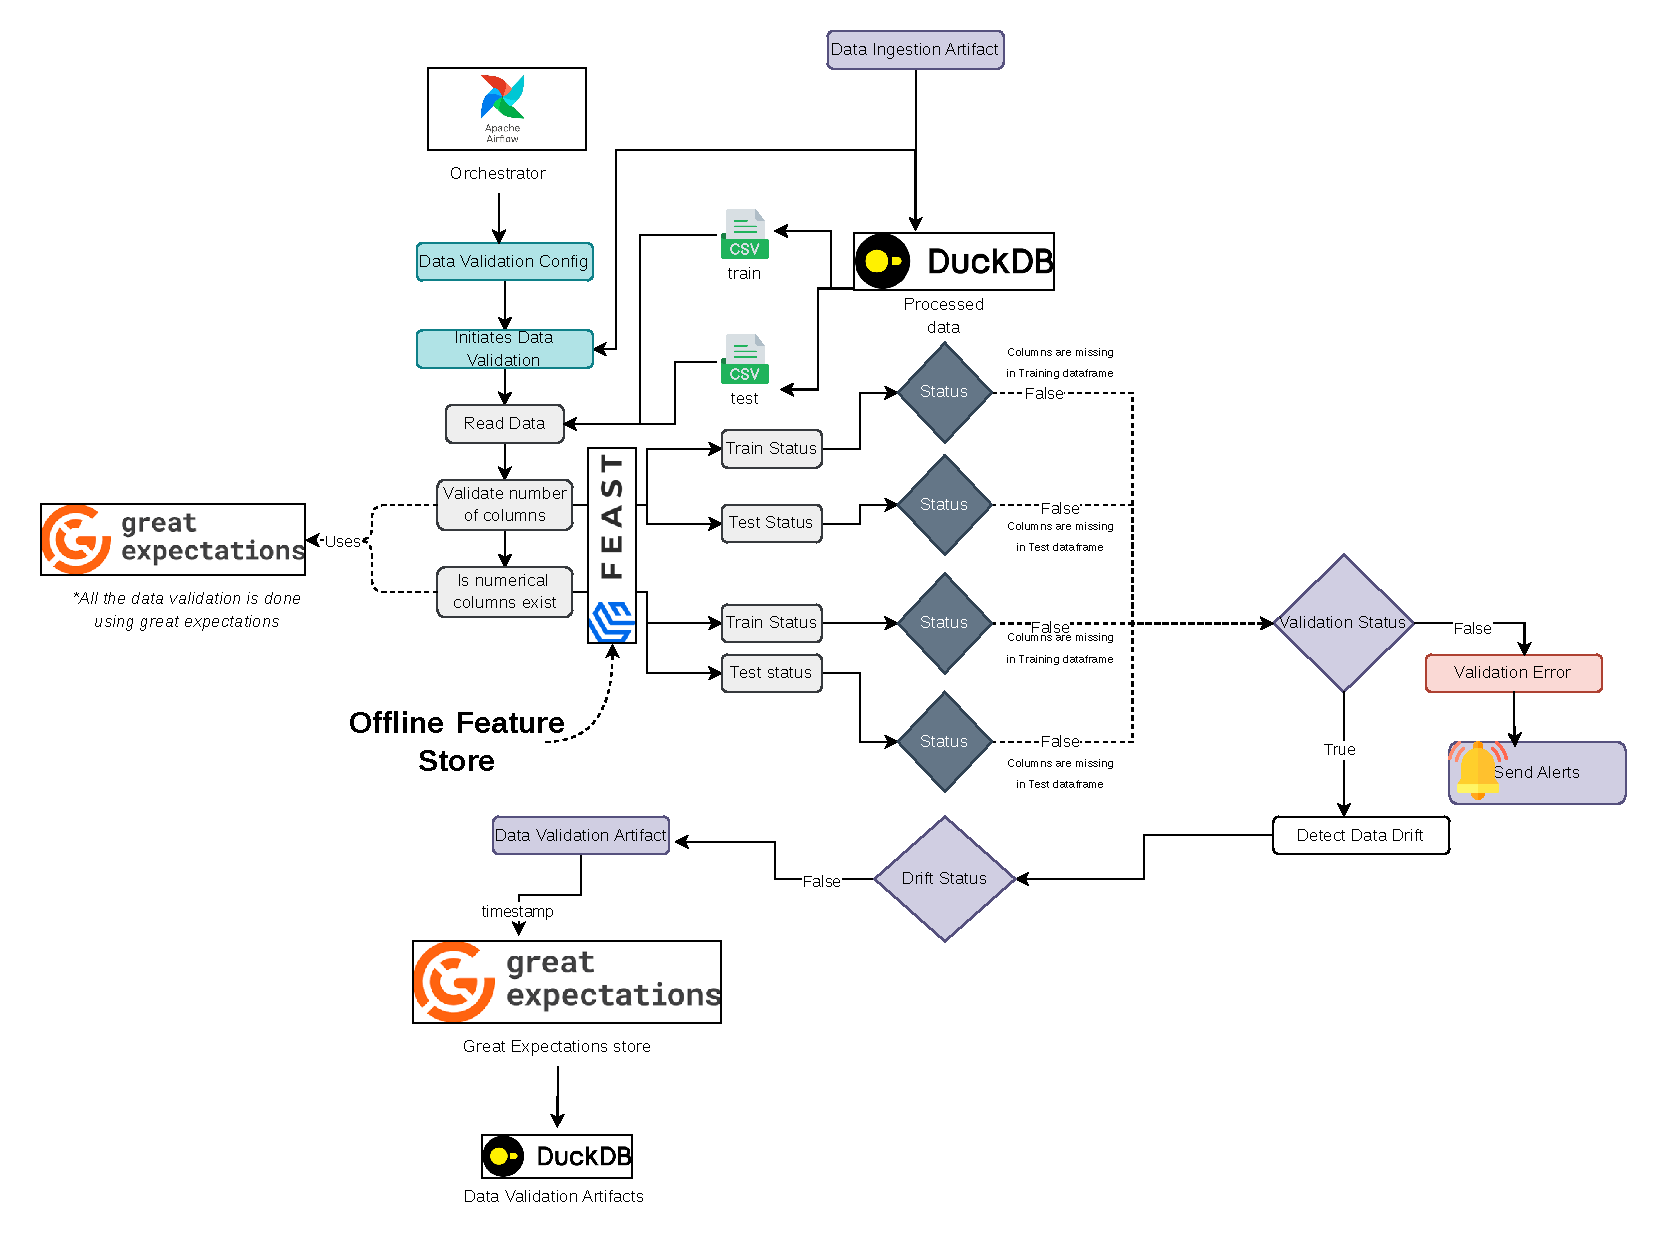
\includegraphics[width=\linewidth,keepaspectratio]{dataValidation.pdf}
  \caption{Pre-processing: validation, feature store, and train/test split under orchestration.}
  \label{fig:preprocessing}
\end{figure}

CSV was tempting for quick plots but punishes wide schemas due to the repetitiveness of nature of data. Each user can play different formats of chess on platform and can also play many games. In our case. The pre-processing stage is where I spent the most calendar time. 




% \subsubsection{Analytical processing angle.} 
% The brief asks how data supports ML and investigation. SQL answers distribution questions (rating histograms, opening popularity by month). The Pandas pipeline encodes domain knowledge (Bullet vs Blitz, title hierarchies). Feast enforces temporal discipline. Together they mean preprocessing is not a single script but a chain where each tool does one job well. When GE fails, I inspect which expectation broke, often a new Lichess header field appeared, and patch transforms before re-running the DAG.

\section{Model development}
\label{sec:model-dev}

\subsection{What}

Model development trains a supervised classifier to predict game outcome from pre-game information such as ratings, titles, time control, opening family, and historical form. The business question that I was tackling was practical, if a player considers a given opening at their rating, what outcome distribution should they expect? Labels are three possible outcomes of white win, black win and draw. Deliverables include \texttt{model.joblib} on disk, metrics JSON, and a registered model in MLflow \parencite{mlflow}.

\subsection{Why}

Game-level rows are the natural ingestion grain, but players think in ``my colour, my rating band, my opening''. \codecite{code_dataset} expands each game to player-centric rows via \texttt{to\_player\_perspective} so the model answers that question.

\subsection{How}

Airflow task "\texttt{train\_model}" calls \texttt{lichess-models train}. Inside \codecite{code_train} where I wrap a scikit-learn \parencite{sklearn} \texttt{Pipeline} \codecite{code_features} which helps in building a \texttt{ColumnTransformer} for numeric and categorical columns, After which a classifier slot searched with \texttt{GridSearchCV} and \texttt{train test split}. Candidate estimators include logistic regression, random forest, and histogram gradient boosting; grids live in \texttt{PARAM\_GRIDS}.

The best pipeline serialises to \texttt{artifacts/lichess\_models/\{run\_id\}/model.joblib}. \codecite{code_evaluate} scores the hold-out split and logs accuracy, macro-F1, and confusion-friendly counts to MLflow. \codecite{code_register} publishes under the name \texttt{lichess-outcome-predictor}. The MLflow stack \githubparencite{code_mlflow_compose} uses Postgres for metadata and MinIO (\texttt{mlflow-artifacts} bucket) for large artefacts, start \texttt{core} and \texttt{ml} profiles together or tracking breaks. I also kept notebooks under \texttt{notebook/} for exploratory work. The CLI path is what Airflow relies on. 

\begin{figure}[htbp]
  \centering
  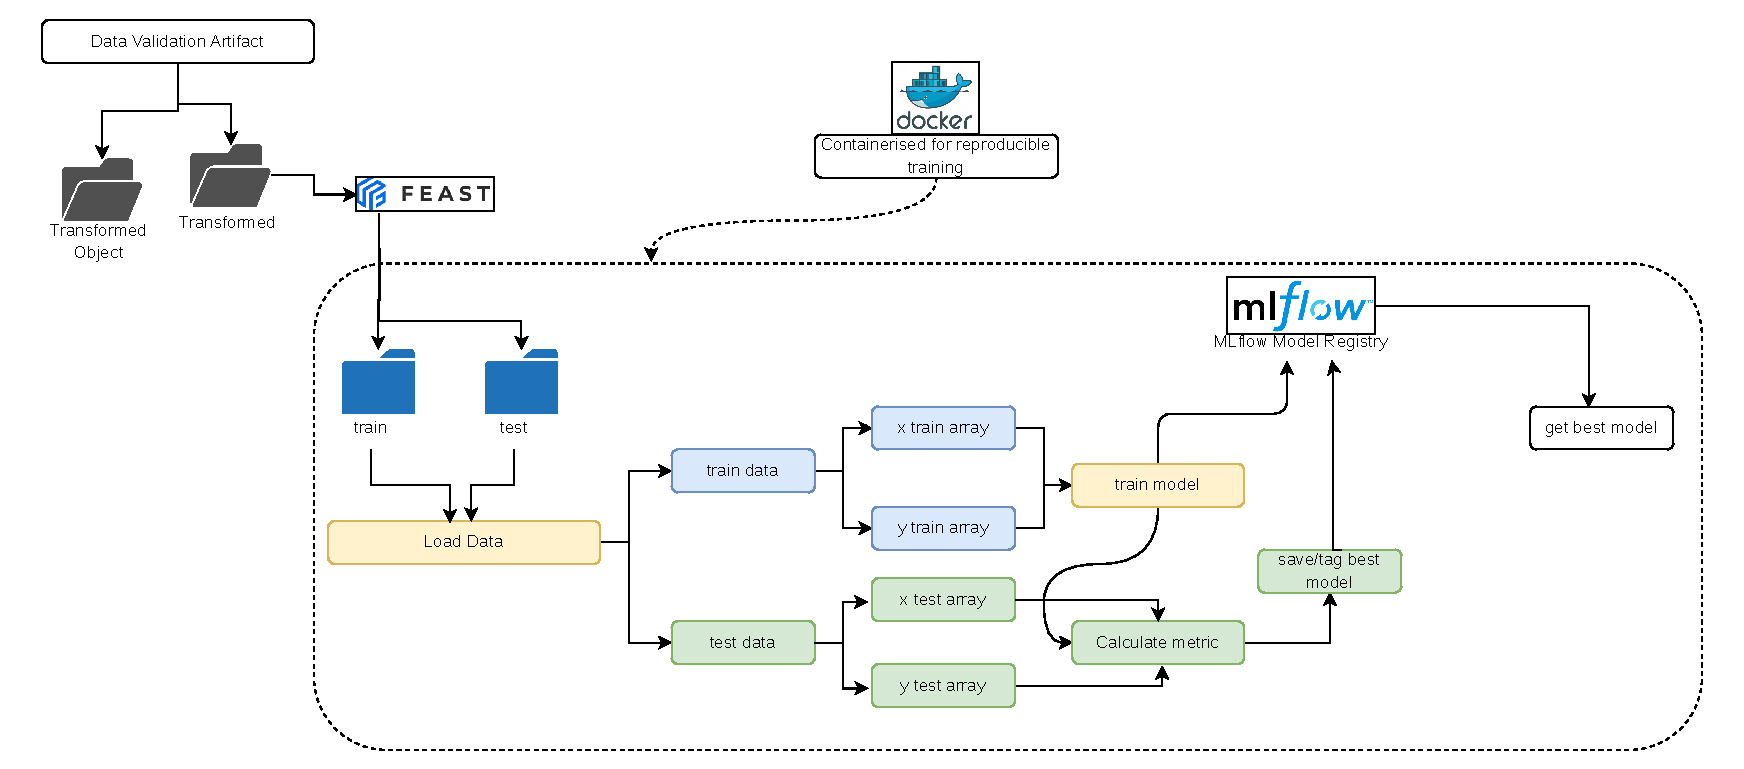
\includegraphics[width=\linewidth,keepaspectratio]{modelTrainer.pdf}
  \caption{Model training: load splits, fit with hyperparameter search, log to MLflow.}
  \label{fig:model-trainer}
\end{figure}

The multi-class framing matches Lichess results better than treating draws as noise. I have not yet wired the opening weakness report (\repo{packages/lichess_models/src/lichess_models/analyze.py}) into the monthly DAG. It remains a manual analysis script for now.

% \textbf{Metrics and reproducibility.} Hold-out evaluation logs accuracy and macro-F1; I watch both because class imbalance makes accuracy optimistic. MLflow stores the conda-free environment implicitly through pip requirements in the repo; I still note the git commit hash manually in run tags when experimenting. For coursework evidence, the combination of \texttt{model.joblib}, MLflow UI screenshots, and cited training code satisfies ``development of ML models'' better than a single accuracy number in this PDF.

% \textbf{Retrieval of training data.} Splits live under artefact paths returned by \texttt{split\_paths(month)} in \codecite{code_dataset}. Airflow passes \texttt{--month} or \texttt{--previous-month} consistently across tasks so training never points at the wrong shard. That sounds obvious, but mismatched month parameters caused a silent train-on-January / evaluate-on-February bug during one all-nighter I do not want to repeat.

\section{Model deployment}
\label{sec:deployment}

\subsection{What}

Deployment here means exposing a trained model over HTTP so another service (or a human with curl) can request predictions without rerunning training. The FastAPI application \parencite{fastapi} in \codecite{code_serving_app} serves \texttt{/health} and \texttt{/predict}. At startup it resolves a model URI \texttt{models:/lichess-outcome-predictor/Staging} from the MLflow registry.

\subsection{Why}

Serialising with \texttt{joblib} is simple. Registering the same object in MLflow ties the running API to an experiment lineage. When April's retrain beats March, It promotes a new version to staging.

\subsection{How}

% \texttt{\_load\_model} runs in the FastAPI lifespan hook. It branches on whether \texttt{MODEL\_URI} ends with \texttt{.joblib} or points at MLflow; the latter downloads the sklearn flavour through the tracking API. Request bodies follow \codecite{code_serving_schemas}: rating, title, time control, opening fields in \texttt{PredictRequest}, with class probabilities and a human-readable outcome label in \texttt{PredictResponse}. \codecite{code_features} supplies \texttt{build\_inference\_row} so training and serving share encoding logic---I fixed a nasty mismatch here once when one-hot columns diverged.

I start the server with \texttt{uv run lichess-serving} from the repo root after exporting \texttt{MODEL\_URI} and MLflow tracking variables. The CLI in \repo{packages/lichess_serving/src/lichess_serving/cli.py} wraps Uvicorn. Containerising is straightforward (slim Python image, same env vars) but left out of this submission to save integration time.

\begin{figure}[htbp]
  \centering
  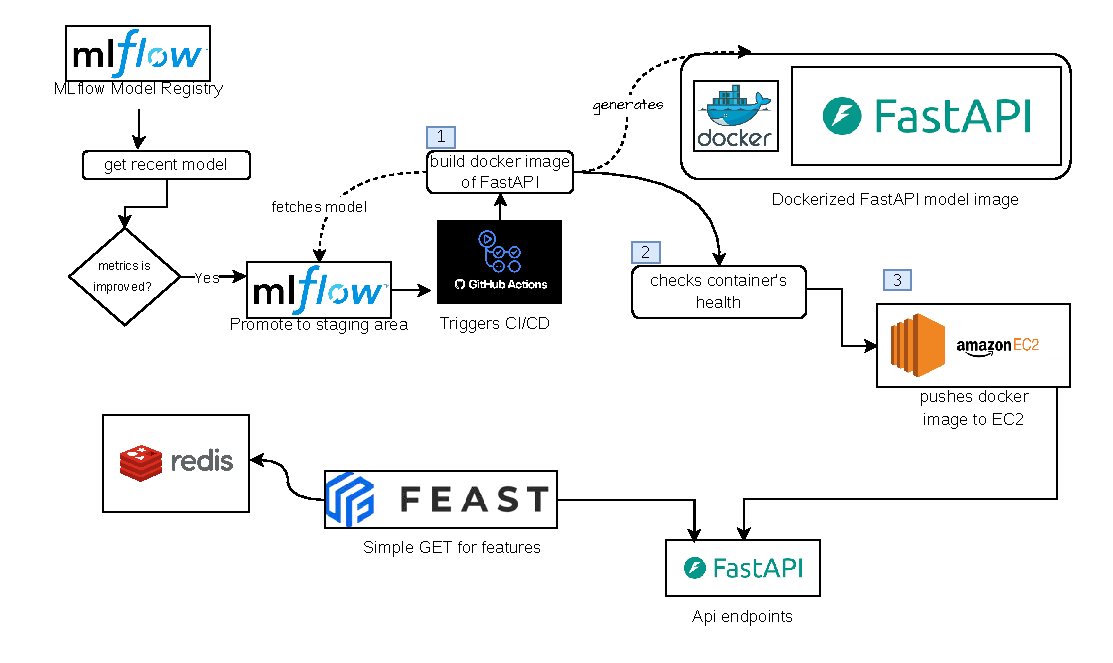
\includegraphics[width=\linewidth,keepaspectratio]{deployment.pdf}
  \caption{Deployment: promote model from MLflow, serve via FastAPI.}
  \label{fig:deployment}
\end{figure}


% \textbf{Serialisation and network access.} The brief asks how models are stored and retrieved. On disk, \texttt{joblib} captures the fitted \texttt{Pipeline}; in MLflow, the same object is versioned with metrics and parameters. Over the network, JSON requests map to Python dicts, pass through the shared preprocessor, and return probabilities---no batch file hand-off. Docker would add an extra layer (image digest, published port 8080, health check in Compose) without changing that contract; I documented the host-run path because it is what I demo today.

\section{Model monitoring}
\label{sec:monitoring}
Accuracy on last month's hold-out does not guarantee next month's performance of model. New openings surge after influencer games; rating inflation drifts feature means. Without metrics, It wouldbe hard to notice serving failures unless a user complains. Monitoring, in my setup, spans three layers which are infrastructure metrics from the API, data-quality re-checks when a new month lands, and drift visualisation. Prometheus \parencite{prometheus} scrapes the serving FastAPI server. Grafana dashboards visualizes using the prometheus. Evidently \parencite{evidently} renders drift reports and other model monitoring reports and this monitoring step runs every day on scheduled time by Airflow's orchestration. Monitoring stage also uses the the slack notification alerts which alerts the team when the problem like data drift or failure happens. 

\begin{figure}[htbp]
  \centering
  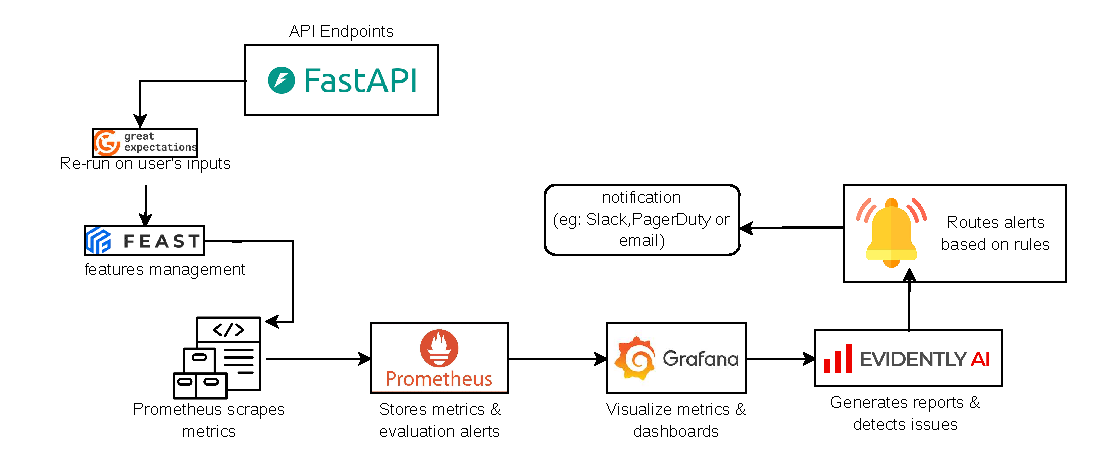
\includegraphics[width=\linewidth,keepaspectratio]{monitoringObserv.pdf}
  \caption{Monitoring: Prometheus, Grafana, drift reports, and pipeline alerts.}
  \label{fig:monitoring}
\end{figure}



\input{content/07-implementation}
\chapter{Reflective Discussion}
\label{ch:reflection-formative}

\begin{figure}[htbp]
  \centering
  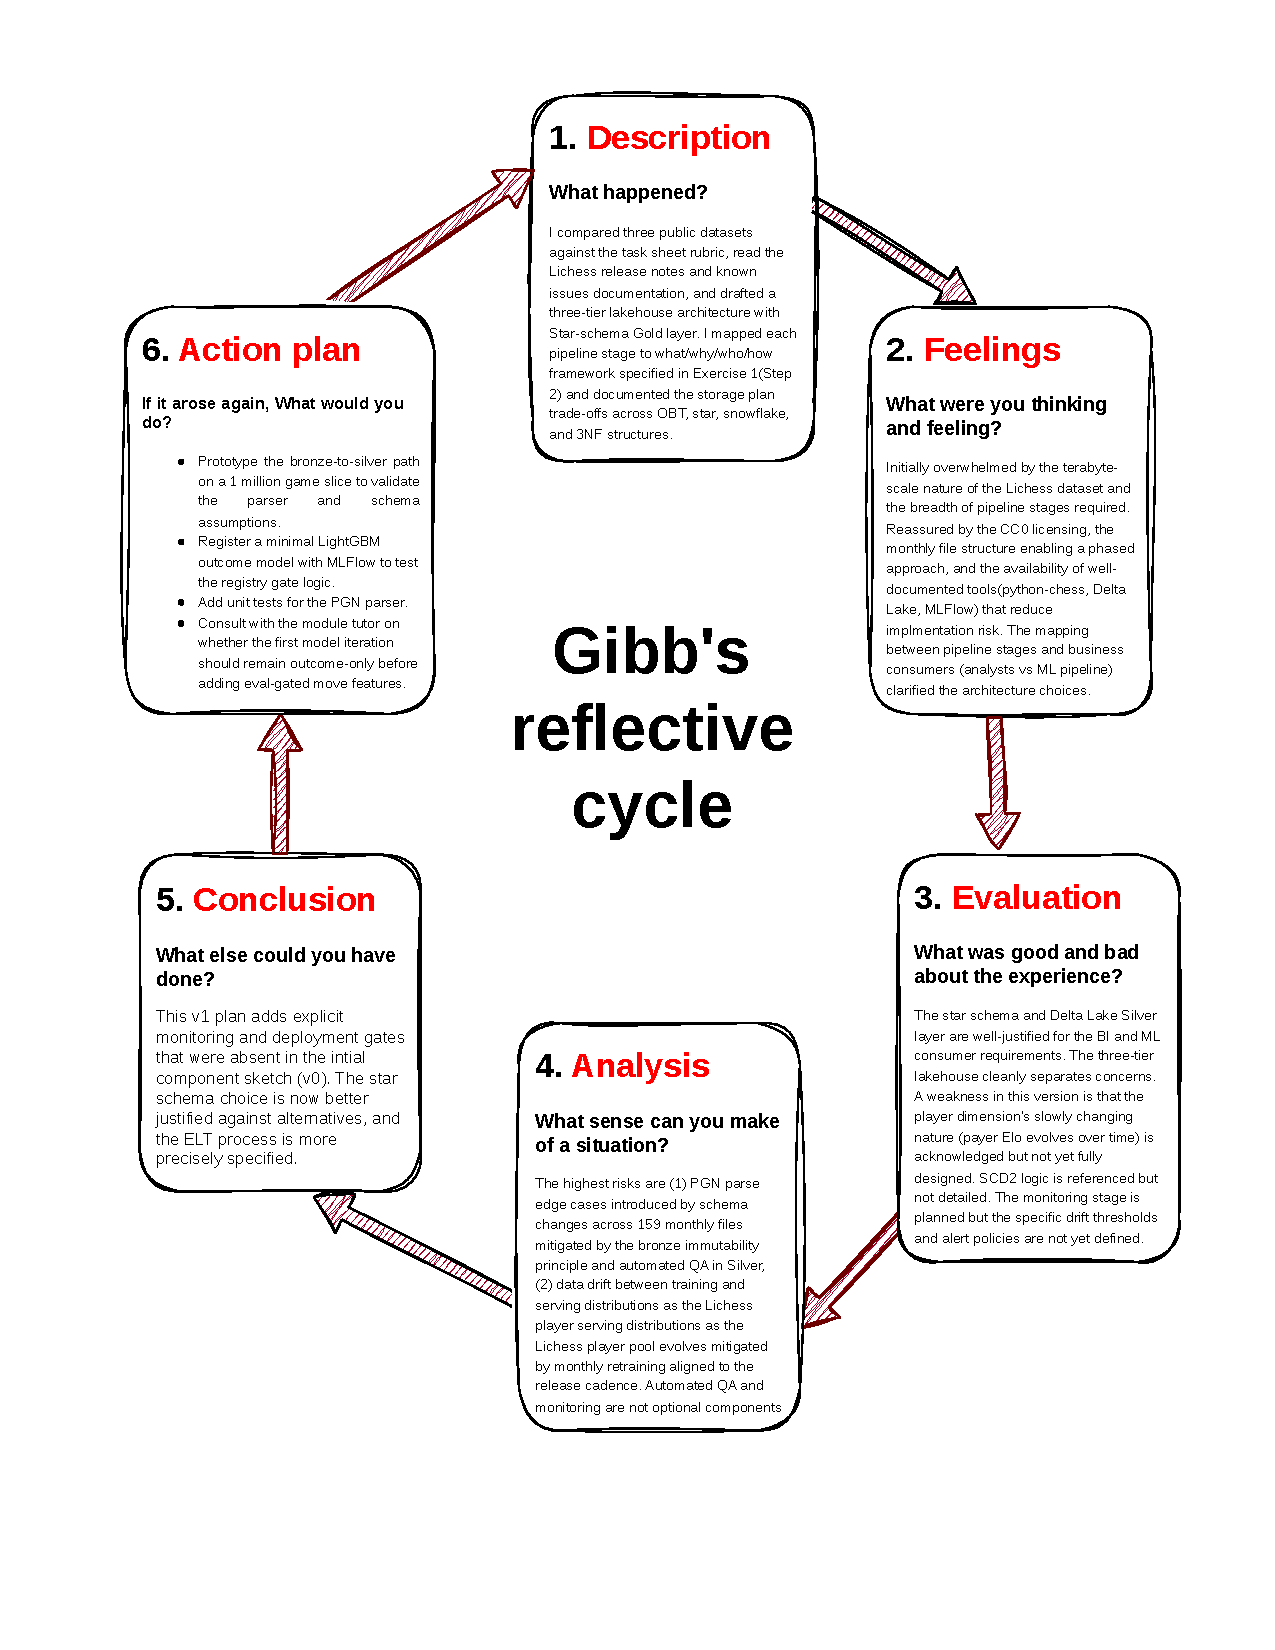
\includegraphics[width=0.95\linewidth,height=0.65\textheight,keepaspectratio]{reflection}
  \caption[Gibb's reflective cycle for iterative MLOps planning.]{\textit{Gibb's reflective cycle} applied to iterative planning and implementation for the Lichess MLOps pipeline.}
  \label{fig:reflection-iterations}
\end{figure}

% Task~1 described a pipeline I had not yet wired: Airflow orchestration, MinIO layers, Spark transform, MariaDB analytics, Feast for temporal features, MLflow registry, FastAPI serving, and Prometheus plus Evidently for observability. The implementation in this repository follows that spine closely. Where the live system diverges, the reasons are mostly resource constraints on a student laptop rather than a change of mind about architecture.

% \textbf{Initial plan versus what I built.} I planned ELT from the start and stuck with it. The surprise was how much shared plumbing (\codecite{code_config_loader}, artefact paths, S3 helpers) mattered before any stage felt finished. I added the \texttt{use\_elt} DAG flag after fighting Spark memory on a single-node cluster; the legacy extract path is not in the original diagram but saved weeks of blocked progress. Config and artefact managers from my early draft notes became real modules instead of remaining bullet points.

% \textbf{Final plan versus gaps.} Serving still runs on the host, not as a Compose service with health checks and rolling updates. Evidently drift is API-triggered: I copy Parquet into \texttt{services/evidently/data/} and call the report endpoint rather than a DAG task firing automatically. Retrain-on-drift is design-only. Great Expectations stores metadata in Postgres while validations execute from the host CLI---fine for demonstration, fragile for a team handover. These gaps are acceptable for coursework marks focused on ``implemented pipeline with evidence,'' but I would close them before calling the system production-ready.

% \textbf{What I would improve next.} Containerise \texttt{lichess-serving} beside MLflow; add an Airflow branch after \texttt{validate\_ge} that calls Evidently and opens an MLflow run when drift exceeds a threshold; promote models through Staging $\rightarrow$ Production with a canary metric gate; wire opening weakness analysis into the API so the player-facing story in my draft is user-visible, not a script. Storage-wise I would document retention on \texttt{lichess-raw} keys (months are large) and test restore from backup.

% Comparing diagrams from Task~1 to this repo, the biggest lesson is iterative refinement the brief emphasises: the written plan was directionally right, but checksum gating, chronological splits, and shared config emerged from debugging real Lichess files, not from the first whiteboard pass.

% \textbf{Discrepancies worth naming.} Task~1 showed decompression inside ingestion; I deferred decompress to Spark or the legacy extract precisely because ELT keeps the raw blob bit-identical to Lichess. Task~1 implied automated alerts to Slack; I rely on Airflow email and log files today. Task~1's monitoring diagram suggested continuous drift scoring; Evidently runs when I invoke it. None of these invalidate the architecture---they are scope cuts I would schedule if this were a team sprint.

% \textbf{Personal takeaway.} Building the pipeline taught me more about data engineering than tuning the classifier. Chess data is messy, large, and interesting; tooling choices (MinIO, MariaDB, Airflow) only earn their keep when retrieval paths and validation gates are boringly reliable. I am satisfied the repository demonstrates implementation depth; the reflection is where I acknowledge what remains stubbed rather than pretending the last ten percent is done.

% \chapter{Further Plans for the Next Submission}
% \label{ch:further-plans}

% In next submission, I will close the gaps identified. The most important are containerising the FastAPI server, automating Evidently drift checks in Airflow, and implementing retrain-on-drift. I will also add a canary metric gate to promote models through Staging to Production and wire opening weakness analysis into the API so the player-facing story in my draft is user-visible, not a script. Storage-wise I would document retention on \texttt{lichess-raw} keys (months are large) and test restore from backup.

%TC:ignore

\appendix

\begingroup
\singlespacing
\small
\setlength{\parskip}{0.25ex plus 0.1ex}
\setlist{nosep,leftmargin=*}
\makeatletter
\renewcommand\section{\@startsection{section}{1}{\z@}{-0.75ex \@plus -0.2ex}{0.4ex}{\normalfont\bfseries\small}}
\makeatother
\chapter{Candidate dataset illustrations}
\label{app:candidate-datasets}

\begin{figure}[htbp]
  \centering
  
\includegraphics[width=\linewidth,keepaspectratio]{lichessSampleFile}
  \caption{Excerpt from a Lichess-rated PGN archive: tournament headers, player ratings, opening metadata, SAN movelist, engine evaluations (\texttt{\%eval}), and clock stamps (\texttt{\%clk}).}
  \label{fig:lichess-pgn-sample}
\end{figure}

\begin{figure}[htbp]
  \centering
  
\includegraphics[width=\linewidth,keepaspectratio]{uci_wine}
  \caption{UCI Wine Quality variable inventory: eleven continuous physicochemical features, ordinal \texttt{quality} target (0--10), and \texttt{color} stratum~\cite{UCIWineQuality}.}
  \label{fig:uci-wine-schema}
\end{figure}

\begin{figure}[htbp]
  \centering
  
\includegraphics[width=0.8\linewidth,keepaspectratio]{bostonHouseprice}
  \caption{Boston housing corpus header and fixed-width numeric rows: fourteen tract-level predictors with \texttt{MEDV} as the regression target~\cite{HarrisonRubinfeld1978,UCIBostonHousing}.}
  \label{fig:boston-housing-sample}
\end{figure}

\chapter{Lichess Open Database (reference material)}
\label{app:lichess-open-database}

This appendix records the public specification of the \textbf{Lichess Open Database} as published on \texttt{database.lichess.org}, together with ingestion-oriented notes that matter when treating monthly PGN shards as pipeline inputs.
The aggregate statistics and inventory table below mirror the project index on \textbf{21 May 2026} (\cref{tab:lichess-monthly-inventory}); later releases will supersede these totals without invalidating the file-level conventions described here.

\section{Licence and redistribution}

Exports are dedicated to the public domain under the Creative Commons \textsc{cc}0~1.0 licence: you may use the data for research, commercial work, publication, or any other purpose, and may download, modify, and redistribute copies without seeking individual permission from the host\footnote{See the licence deed \cite{cc0_10}; catalogue page \cite{lichess_open_database}.}.

\section{Branding and catalogue context}

\noindent
Figure~\ref{fig:lichess-appendix-logo} is reserved for the Lichess wordmark as used in database collateral (drop a vector \textsc{pdf} into the path named in the figure).
Figure~\ref{fig:lichess-appendix-database-page} is reserved for a cropped screenshot of the standard-rated games index if you wish to show the live download table in context.
Both figures are optional; the appendix remains complete if you omit the artwork but retain the captions, which carry the scholarly attribution.

\begin{figure}[htbp]
  \centering
  \IfFileExists{figures/appendix/lichess-logo.pdf}{%
    \includegraphics[height=16mm]{lichess-logo.pdf}}{%
    \fbox{\begin{minipage}[c][0.14\textheight][c]{0.58\linewidth}\centering\small\itshape
    Place the Lichess wordmark here as \texttt{figures/appendix/lichess-logo.pdf}.\\
    Use vector artwork from official press or brand assets where possible.
    \end{minipage}}}
  \caption{Lichess wordmark (placeholder until artwork is embedded). The public database index presents this mark in its header; embedding the mark signals the data source for readers. Source: \cite{lichess_open_database}.}
  \label{fig:lichess-appendix-logo}
\end{figure}

\begin{figure}[htbp]
  \centering
  \IfFileExists{figures/appendix/lichess-database-index.png}{%
    \includegraphics[width=0.92\linewidth]{lichess-database-index.png}}{%
    \IfFileExists{figures/appendix/lichess-database-index.pdf}{%
      \includegraphics[width=0.92\linewidth]{lichess-database-index.pdf}}{%
    \fbox{\begin{minipage}[c][0.22\textheight][c]{0.92\linewidth}\centering\small\itshape
    Optional: add a cropped screenshot of \texttt{database.lichess.org} (\texttt{figures/appendix/lichess-database-index.png} or \texttt{.pdf}).\\
    Crop to the standard-rated games panel so Month\,/\,Size\,/\,Games remain legible.
    \end{minipage}}}}
  \caption{Optional depiction of the standard-rated-games download index (replace placeholder when a screenshot is available). Demonstrates where monthly \texttt{.pgn.zst} and BitTorrent pointers are maintained. Source: \cite{lichess_open_database}.}
  \label{fig:lichess-appendix-database-page}
\end{figure}

\section{Corpus scope (standard rated games)}

The \emph{standard rated} subset consists of \(7{,}772{,}124{,}731\) games played on \texttt{lichess.org} and serialised as \textsc{pgn}.
Each monthly file is \emph{non-cumulative}: it contains only the games whose clock time falls in that calendar month.
Across history the release set spans \textbf{160} monthly files with a combined compressed footprint of approximately \textbf{2.46\,TB}.
Parallel exports exist for variants, broadcasts, puzzles, and evaluations; this report focuses on standard chess rated games and points readers to the same catalogue page for sibling products \cite{lichess_open_database}.

\section{Monthly export inventory}

\noindent
Monthly files ship as Zstandard-compressed PGN (\texttt{.pgn.zst}); the project page also mirrors BitTorrent payloads for bulk retrieval.
Plain-text download manifests and \textsc{sha}256 checksums are published alongside the artefacts (retrieve from the index rather than copying digests into this PDF).

{\footnotesize
\begin{longtable}{@{}l r r@{}}
  \caption{Monthly standard-rated Lichess corpora (compressed containers).}%
  \label{tab:lichess-monthly-inventory}\\
  \toprule
  Month & Size & Games \\
  \midrule
  \endfirsthead
  \caption[]{\textit{(continued)} Monthly standard-rated Lichess corpora.}\\
  \toprule
  Month & Size & Games \\
  \midrule
  \endhead
  \midrule
  \multicolumn{3}{r}{\textit{Continued on next page}}\\
  \endfoot
  2026 -- April & 29.3 GB & 89\,962\,564 \\
2026 -- March & 29.4 GB & 90\,074\,196 \\
2026 -- February & 27.8 GB & 84\,600\,043 \\
2026 -- January & 30.7 GB & 94\,604\,722 \\
2025 -- December & 30.8 GB & 94\,847\,276 \\
2025 -- November & 29.4 GB & 90\,633\,152 \\
2025 -- October & 29.9 GB & 91\,549\,148 \\
2025 -- September & 28.3 GB & 87\,049\,890 \\
2025 -- August & 30.2 GB & 92\,695\,519 \\
2025 -- July & 30.4 GB & 93\,092\,772 \\
2025 -- June & 29.7 GB & 91\,189\,178 \\
2025 -- May & 30.7 GB & 94\,068\,115 \\
2025 -- April & 29.8 GB & 91\,757\,350 \\
2025 -- March & 31.8 GB & 97\,512\,351 \\
2025 -- February & 29.2 GB & 89\,430\,612 \\
2025 -- January & 32.9 GB & 100\,412\,379 \\
2024 -- December & 31.6 GB & 96\,587\,411 \\
2024 -- November & 29.6 GB & 90\,847\,982 \\
2024 -- October & 30.7 GB & 94\,254\,891 \\
2024 -- September & 28.6 GB & 87\,713\,219 \\
2024 -- August & 30 GB & 92\,198\,878 \\
2024 -- July & 29.3 GB & 90\,106\,180 \\
2024 -- June & 29.1 GB & 89\,342\,529 \\
2024 -- May & 30.7 GB & 94\,400\,051 \\
2024 -- April & 29.6 GB & 91\,377\,787 \\
2024 -- March & 31.1 GB & 95\,804\,114 \\
2024 -- February & 29.8 GB & 91\,567\,975 \\
2024 -- January & 32.4 GB & 98\,994\,760 \\
2023 -- December & 31.7 GB & 96\,909\,211 \\
2023 -- November & 30 GB & 92\,389\,636 \\
2023 -- October & 30.8 GB & 94\,922\,297 \\
2023 -- September & 30.3 GB & 93\,218\,629 \\
2023 -- August & 31.2 GB & 96\,118\,124 \\
2023 -- July & 30.8 GB & 95\,300\,285 \\
2023 -- June & 31.2 GB & 96\,641\,906 \\
2023 -- May & 33.7 GB & 104\,193\,153 \\
2023 -- April & 32.9 GB & 101\,706\,224 \\
2023 -- March & 34.9 GB & 108\,201\,825 \\
2023 -- February & 31.8 GB & 98\,471\,537 \\
2023 -- January & 33.5 GB & 103\,178\,407 \\
2022 -- December & 30.2 GB & 93\,501\,009 \\
2022 -- November & 28.9 GB & 89\,319\,297 \\
2022 -- October & 30 GB & 92\,629\,656 \\
2022 -- September & 28.9 GB & 89\,174\,810 \\
2022 -- August & 30 GB & 92\,670\,440 \\
2022 -- July & 29.8 GB & 92\,055\,571 \\
2022 -- June & 28.3 GB & 87\,649\,571 \\
2022 -- May & 28.8 GB & 89\,300\,578 \\
2022 -- April & 28.1 GB & 87\,200\,457 \\
2022 -- March & 29.4 GB & 91\,140\,030 \\
2022 -- February & 28 GB & 86\,339\,501 \\
2022 -- January & 33.2 GB & 102\,110\,423 \\
2021 -- December & 31.1 GB & 95\,600\,810 \\
2021 -- November & 28.2 GB & 87\,113\,345 \\
2021 -- October & 28.5 GB & 88\,092\,721 \\
2021 -- September & 28.5 GB & 88\,133\,339 \\
2021 -- August & 30.4 GB & 93\,679\,328 \\
2021 -- July & 29.8 GB & 92\,193\,352 \\
2021 -- June & 29.7 GB & 92\,190\,803 \\
2021 -- May & 32.7 GB & 101\,011\,629 \\
2021 -- April & 32.1 GB & 99\,184\,138 \\
2021 -- March & 32.4 GB & 100\,023\,791 \\
2021 -- February & 28.9 GB & 89\,892\,001 \\
2021 -- January & 30.8 GB & 95\,853\,038 \\
2020 -- December & 26.6 GB & 89\,422\,803 \\
2020 -- November & 23.2 GB & 78\,268\,317 \\
2020 -- October & 20.9 GB & 70\,572\,373 \\
2020 -- September & 20.1 GB & 68\,027\,862 \\
2020 -- August & 21.2 GB & 71\,405\,167 \\
2020 -- July & 21.1 GB & 70\,592\,022 \\
2020 -- June & 21.1 GB & 70\,374\,749 \\
2020 -- May & 22.8 GB & 75\,628\,855 \\
2020 -- April & 22.2 GB & 73\,224\,608 \\
2020 -- March & 16.6 GB & 55\,544\,817 \\
2020 -- February & 12.9 GB & 44\,004\,185 \\
2020 -- January & 13.7 GB & 46\,800\,709 \\
2019 -- December & 12.9 GB & 44\,055\,757 \\
2019 -- November & 11.8 GB & 40\,357\,832 \\
2019 -- October & 11.9 GB & 40\,440\,254 \\
2019 -- September & 10.9 GB & 36\,996\,010 \\
2019 -- August & 10.8 GB & 36\,745\,427 \\
2019 -- July & 10.5 GB & 35\,728\,182 \\
2019 -- June & 9.98 GB & 33\,935\,786 \\
2019 -- May & 10.3 GB & 35\,236\,588 \\
2019 -- April & 9.87 GB & 33\,565\,536 \\
2019 -- March & 10.3 GB & 34\,869\,171 \\
2019 -- February & 9.17 GB & 31\,023\,718 \\
2019 -- January & 10.1 GB & 33\,886\,899 \\
2018 -- December & 9.3 GB & 31\,179\,146 \\
2018 -- November & 7.81 GB & 26\,136\,657 \\
2018 -- October & 7.39 GB & 24\,784\,600 \\
2018 -- September & 6.84 GB & 22\,971\,939 \\
2018 -- August & 6.81 GB & 22\,635\,642 \\
2018 -- July & 6.34 GB & 21\,070\,917 \\
2018 -- June & 6.09 GB & 20\,273\,737 \\
2018 -- May & 6.46 GB & 21\,442\,600 \\
2018 -- April & 6.02 GB & 19\,881\,929 \\
2018 -- March & 6.57 GB & 20\,059\,178 \\
2018 -- February & 5.28 GB & 17\,383\,410 \\
2018 -- January & 5.47 GB & 17\,945\,784 \\
2017 -- December & 4.95 GB & 16\,232\,215 \\
2017 -- November & 4.36 GB & 14\,306\,375 \\
2017 -- October & 4.18 GB & 13\,703\,878 \\
2017 -- September & 3.83 GB & 12\,564\,109 \\
2017 -- August & 3.81 GB & 12\,458\,761 \\
2017 -- July & 3.69 GB & 12\,080\,314 \\
2017 -- June & 3.52 GB & 11\,512\,600 \\
2017 -- May & 3.59 GB & 11\,693\,919 \\
2017 -- April & 3.48 GB & 11\,348\,506 \\
2017 -- March & 2.17 GB & 11\,346\,745 \\
2017 -- February & 1.8 GB & 10\,194\,939 \\
2017 -- January & 1.9 GB & 10\,680\,708 \\
2016 -- December & 1.7 GB & 9\,433\,412 \\
2016 -- November & 1.44 GB & 8\,021\,509 \\
2016 -- October & 1.35 GB & 7\,599\,868 \\
2016 -- September & 1.21 GB & 6\,813\,113 \\
2016 -- August & 1.16 GB & 6\,483\,257 \\
2016 -- July & 1.12 GB & 6\,275\,933 \\
2016 -- June & 1.09 GB & 6\,136\,419 \\
2016 -- May & 1.11 GB & 6\,225\,957 \\
2016 -- April & 1.06 GB & 5\,922\,667 \\
2016 -- March & 1.04 GB & 5\,801\,234 \\
2016 -- February & 908 MB & 5\,015\,361 \\
2016 -- January & 872 MB & 4\,770\,357 \\
2015 -- December & 758 MB & 4\,161\,162 \\
2015 -- November & 667 MB & 3\,595\,776 \\
2015 -- October & 647 MB & 3\,400\,418 \\
2015 -- September & 547 MB & 2\,844\,677 \\
2015 -- August & 504 MB & 2\,621\,861 \\
2015 -- July & 483 MB & 2\,455\,141 \\
2015 -- June & 432 MB & 2\,324\,106 \\
2015 -- May & 392 MB & 2\,137\,557 \\
2015 -- April & 317 MB & 1\,785\,418 \\
2015 -- March & 324 MB & 1\,742\,733 \\
2015 -- February & 283 MB & 1\,495\,553 \\
2015 -- January & 286 MB & 1\,497\,237 \\
2014 -- December & 259 MB & 1\,350\,176 \\
2014 -- November & 228 MB & 1\,209\,291 \\
2014 -- October & 205 MB & 1\,111\,302 \\
2014 -- September & 179 MB & 1\,000\,056 \\
2014 -- August & 193 MB & 1\,013\,294 \\
2014 -- July & 200 MB & 1\,048\,440 \\
2014 -- June & 182 MB & 961\,868 \\
2014 -- May & 172 MB & 905\,374 \\
2014 -- April & 137 MB & 810\,463 \\
2014 -- March & 129 MB & 795\,173 \\
2014 -- February & 113 MB & 692\,394 \\
2014 -- January & 111 MB & 697\,600 \\
2013 -- December & 91.8 MB & 578\,262 \\
2013 -- November & 77 MB & 487\,012 \\
2013 -- October & 62.7 MB & 411\,039 \\
2013 -- September & 47.2 MB & 325\,098 \\
2013 -- August & 47.7 MB & 325\,525 \\
2013 -- July & 43 MB & 293\,459 \\
2013 -- June & 32.9 MB & 224\,679 \\
2013 -- May & 26.5 MB & 179\,550 \\
2013 -- April & 23.3 MB & 157\,871 \\
2013 -- March & 23.6 MB & 158\,635 \\
2013 -- February & 18.2 MB & 123\,961 \\
2013 -- January & 17.8 MB & 121\,332 \\
\midrule
\textbf{Total} & \textbf{2.46 TB} & \textbf{7\,772\,124\,731} \\
\bottomrule

\end{longtable}
}

\section[Format example]{Illustrative record (\textsc{pgn})}

The following excerpt (abridged only where noted) illustrates typical header tags, embedded Stockfish evaluation comments from White's point of view, and clock annotations.

\begin{lstlisting}[language=PGN,label={lst:lichess-pgn-sample}, basicstyle=\ttfamily\scriptsize, columns=fullflexible, keepspaces=true, aboveskip=0.75em, belowskip=0.75em]
[Event "Rated Bullet tournament https://lichess.org/tournament/yc1WW2Ox"]
[Site "https://lichess.org/PpwPOZMq"]
[Date "2017.04.01"]
[Round "-"]
[White "Abbot"]
[Black "Costello"]
[Result "0-1"]
[UTCDate "2017.04.01"]
[UTCTime "11:32:01"]
[WhiteElo "2100"]
[BlackElo "2000"]
[WhiteRatingDiff "-4"]
[BlackRatingDiff "+1"]
[WhiteTitle "FM"]
[ECO "B30"]
[Opening "Sicilian Defense: Old Sicilian"]
[TimeControl "300+0"]
[Termination "Time forfeit"]

1. e4 { [%eval 0.17] [%clk 0:00:30] } 1... c5 { [%eval 0.19] [%clk 0:00:30] }
2. Nf3 { [%eval 0.25] [%clk 0:00:29] } 2... Nc6 { [%eval 0.33] [%clk 0:00:30] }
3. Bc4 { [%eval -0.13] [%clk 0:00:28] } 3... e6 { [%eval -0.04] [%clk 0:00:30] }
4. c3 { [%eval -0.4] [%clk 0:00:27] } 4... b5? { [%eval 1.18] [%clk 0:00:30] }
5. Bb3?! { [%eval 0.21] [%clk 0:00:26] } 5... c4 { [%eval 0.32] [%clk 0:00:29] }
6. Bc2 { [%eval 0.2] [%clk 0:00:25] } 6... a5 { [%eval 0.6] [%clk 0:00:29] }
7. d4 { [%eval 0.29] [%clk 0:00:23] } 7... cxd3 { [%eval 0.6] [%clk 0:00:27] }
8. Qxd3 { [%eval 0.12] [%clk 0:00:22] } 8... Nf6 { [%eval 0.52] [%clk 0:00:26] }
9. e5 { [%eval 0.39] [%clk 0:00:21] } 9... Nd5 { [%eval 0.45] [%clk 0:00:25] }
10. Bg5?! { [%eval -0.44] [%clk 0:00:18] } 10... Qc7 { [%eval -0.12] [%clk 0:00:23] }
11. Nbd2?? { [%eval -3.15] [%clk 0:00:14] } 11... h6 { [%eval -2.99] [%clk 0:00:23] }
12. Bh4 { [%eval -3.0] [%clk 0:00:11] } 12... Ba6? { [%eval -0.12] [%clk 0:00:23] }
13. b3?? { [%eval -4.14] [%clk 0:00:02] } 13... Nf4? { [%eval -2.73] [%clk 0:00:21] } 0-1
\end{lstlisting}

\section{Technical notes for preprocessing}

\begin{itemize}[leftmargin=2em]
  \item Roughly 6\% of games embed Stockfish analysis markers such as \texttt{[\%eval 2.35]} (centipawn advantage) or mate-distance hashes like \texttt{\#-4}; evaluations read from White's perspective.
  \item \texttt{WhiteElo} and \texttt{BlackElo} encode Glicko-2 ratings as published by Lichess.
  \item Clock telemetry appears as \texttt{\%clk} comments to the second from April~2017 onward; a historical export (\texttt{\%clkc}) exists for centisecond precision on older coverage.
  \item Accounts driven through the Bot \textsc{api} expose \texttt{[WhiteTitle "BOT"]} or \texttt{[BlackTitle "BOT"]}.
  \item Non-standard rule sets include a \texttt{Variant} tag (for example \texttt{Antichess}).
  \item \textbf{Zstandard:} Unix users may run \texttt{pzstd -d file.pgn.zst}; Windows users commonly rely on PeaZip or equivalent. Uncompressed text is roughly \(7.1\times\) larger than the \texttt{.zst}.
  \item Partial downloads support partial decompression; pipe decompression streams directly into analytical scripts (\texttt{zstdcat} into Python, for example) to avoid writing fully expanded copies to disk.
  \item Interactive database tools (\textsc{scid}, ChessBase) often struggle with single multi-terabyte \textsc{pgn} files; split files or programmatic parsers (python-chess, Scoutfish) are the practical route.
\end{itemize}

\section{Documented data-quality caveats}

These items summarise known regressions and anomalies published alongside the database; treat them as schema- and era-dependent limitations when training or auditing models.

\begin{description}[style=nextline,font=\normalfont\bfseries,leftmargin=0.7cm]
  \item[November 2023] Some Chess960 rematches record invalid castling rights in the starting \textsc{fen}.
  \item[December 2022] Some Antichess rows carry bullet ratings in error.
  \item[12 March 2021] Result tags may be wrong for a subset affected by a database outage after a datacentre incident.
  \item[9 February 2021] Resignations can appear after the recorded terminal position; variant games may list moves past the decisive moment.
  \item[December 2020 / January 2021] Many variant games were analysed with standard \textsc{nnue} settings, yielding incorrect evaluations.
  \item[Up to December 2020] Some exports omit redundant yet normative headers (for example \texttt{Round}), omit \texttt{Date} (use \texttt{UTCDate}/\texttt{UTCTime}), or drop black move numbers after comments---later re-exports may repair this.
  \item[July--August 2020] Large swathes (notably 31~July) show unreliable opening evaluations for variants (up to fifteen plies).
  \item[December 2016 (peak 9th)] Widespread evaluation corruption.
  \item[Before 2016] Mate-distance comments do not always correspond to true mates.
  \item[June 2020; before March 2016] Rated self-play was possible in isolated cases.
  \item[Up to August 2016] Seven games contain illegal castling moves in the move list.
\end{description}

\section{Community derivatives}

Lichess maintains a curated, evolving list of research projects and derivative tools built atop these releases.
Rather than reproducing brittle URLs here, consult the live catalogue on \texttt{database.lichess.org}, which stays current as new work appears\cite{lichess_open_database}.

\section*{Feedback}

The maintainers invite researchers to share derived results via \href{mailto:contact@lichess.org}{\texttt{contact@lichess.org}} (\cite{lichess_open_database}).

\section{Code index}
\label{app:code-index}

Table~\ref{tab:code-index} lists major implementation files with GitHub links (\githubicon). All paths are relative to repository root on branch \texttt{main}.

{\small
\begin{longtable}{@{}p{0.36\linewidth}p{0.52\linewidth}@{}}
\toprule
\textbf{File} & \textbf{Description} \\
\midrule
\endhead
\repo{libs/shared/config_loader.py} & YAML config merge \\
\repo{libs/shared/artifact_manager.py} & Artefact path resolution \\
\repo{libs/shared/s3.py} & MinIO/S3 client helpers \\
\repo{libs/shared/storage_config.py} & MariaDB and S3 URI mapping \\
\repo{libs/shared/logger.py} & Rotating file logging \\
\repo{services/airflow/dags/lichess_monthly_ingestion.py} & Monthly orchestration DAG \\
\repo{packages/lichess_data/src/lichess_data/extract/lichess_downloader.py} & Shard download and checksum \\
\repo{packages/lichess_data/src/lichess_data/validate/checks.py} & SHA256 validation \\
\repo{packages/lichess_data/src/lichess_data/load/upload.py} & Raw upload to MinIO \\
\repo{services/minio/docker-compose.yml} & Object store and buckets \\
\repo{packages/lichess_data/src/lichess_data/spark/transform.py} & Spark star-schema transform \\
\repo{packages/lichess_data/src/lichess_data/load/MariaDB_sync.py} & Parquet $\rightarrow$ MariaDB sync \\
\repo{packages/lichess_data/src/lichess_data/preprocessing/transforms.py} & Pandas feature stages \\
\repo{packages/lichess_data/src/lichess_data/extract/pgn_parser.py} & Legacy PGN parser \\
\repo{packages/lichess_features/src/lichess_features/split.py} & Feast split and temporal cut \\
\repo{packages/lichess_data/src/lichess_data/validate/ge_runner.py} & Great Expectations runner \\
\repo{packages/lichess_models/src/lichess_models/train.py} & Hyperparameter search training \\
\repo{packages/lichess_models/src/lichess_models/features.py} & Sklearn preprocessor \\
\repo{packages/lichess_models/src/lichess_models/dataset.py} & Train/test loading \\
\repo{packages/lichess_models/src/lichess_models/evaluate.py} & Hold-out metrics \\
\repo{packages/lichess_models/src/lichess_models/register.py} & MLflow registration \\
\repo{services/mlflow/docker-compose.yml} & MLflow tracking server \\
\repo{packages/lichess_serving/src/lichess_serving/app.py} & FastAPI predict API \\
\repo{packages/lichess_serving/src/lichess_serving/schemas.py} & API request/response models \\
\repo{services/prometheus/prometheus.yml} & Metrics scrape config \\
\repo{services/evidently/src/app_fastapi/main.py} & Drift report API \\
\bottomrule
\caption{Implementation code index with GitHub links.}
\label{tab:code-index}
\end{longtable}
}

\endgroup

\printbibliography[heading=bibintoc]
%TC:endignore

\end{document}
